\documentclass[12pt,a4paper]{report}

% ---------- Paket dasar ----------
\usepackage[utf8]{inputenc}
\usepackage[T1]{fontenc}
\usepackage[indonesian]{babel}
\addto\captionsindonesian{\renewcommand{\bibname}{Referensi}}

% ---------- Paket matematika & gambar ----------
\usepackage{amsmath,amssymb}
\usepackage{graphicx}
\usepackage{caption}
\usepackage{subcaption}
\usepackage{float}
\bibliographystyle{IEEEtran}
% \bstctlcite berasal dari kelas IEEEtran; didefinisikan ulang karena dokumen ini memakai kelas report.
% Dipakai untuk mematikan garis pengganti nama penulis yang berulang di daftar referensi.
\makeatletter
\def\bstctlcite{\@ifnextchar[{\@bstctlcite}{\@bstctlcite[@auxout]}}
\def\@bstctlcite[#1]#2{\@bsphack\@for\@citeb:=#2\do{%
  \edef\@citeb{\expandafter\@firstofone\@citeb}%
  \if@filesw\immediate\write\csname #1\endcsname{\string\citation{\@citeb}}\fi}%
  \@esphack}
\makeatother

% ---------- Paket lain ----------
\usepackage[most]{tcolorbox}
\usepackage{hyperref}
\usepackage{fancyhdr}
\usepackage{titlesec}
\usepackage{longtable}
\usepackage{array}
\usepackage{booktabs}
\usepackage{multirow}
\usepackage[table]{xcolor}
\usepackage{listings}
\usepackage{enumitem}
\usepackage{adjustbox}
\emergencystretch=3em

\setlength{\headheight}{10pt}
\setlength{\headsep}{55pt}
\setlength{\footskip}{28pt}
\usepackage[a4paper,top=3cm,bottom=3cm,left=3cm,right=3cm]{geometry}

% Gambar dari folder public dan dari folder output repository
\graphicspath{{public/}{../output/}}

% ---------- Listing kode Python ----------
\lstdefinestyle{py}{
	language=Python,
	basicstyle=\ttfamily\scriptsize,
	keywordstyle=\color{blue!70!black}\bfseries,
	commentstyle=\color{gray}\itshape,
	stringstyle=\color{teal!70!black},
	numbers=left,
	numberstyle=\tiny\color{gray},
	frame=single,
	rulecolor=\color{gray!50},
	breaklines=true,
	showstringspaces=false,
	tabsize=4,
	columns=fullflexible,
	keepspaces=true,
}
\lstset{style=py}
\renewcommand{\lstlistingname}{Kode}

% --- Pengaturan header & footer ---
\pagestyle{fancy}
\fancyhf{}

\fancypagestyle{plain}{%
	\fancyhf{}%
	\fancyhead[L]{%
		
\includegraphics[height=1.1cm]{logo-itb}\hspace{0.3cm}%
		
\includegraphics[height=1.1cm]{logo-stei}\hspace{0.3cm}%
	}%
	\fancyhead[R]{%
		\begin{minipage}{9cm}
			\raggedleft\bfseries IF3170 Inteligensi Artifisial\\
			\normalsize Laporan Tugas Besar 1\\
			\itshape Semester I 2026/2027
		\end{minipage}
	}%
	\renewcommand{\headrulewidth}{0.4pt}%
	\fancyfoot[L]{\small v1.0}%
	\fancyfoot[C]{\small Halaman \thepage}%
	\fancyfoot[R]{\small }%
	\renewcommand{\footrulewidth}{0.4pt}%
}

\fancyhead[L]{%
	
\includegraphics[height=1.5cm]{logo-itb}\hspace{0.3cm}%
	
\includegraphics[height=1.5cm]{logo-stei}\hspace{0.3cm}%
}

\fancyhead[R]{%
	\begin{minipage}{9cm}
		\raggedleft\bfseries IF3170 Inteligensi Artifisial\\
		\normalsize Laporan Tugas Besar 1\\
		\itshape Semester I 2026/2027
	\end{minipage}
}

\renewcommand{\headrulewidth}{0.4pt}
\fancyfoot[L]{\small v1.0}
\fancyfoot[C]{\small Halaman \thepage}
\fancyfoot[R]{\small }
\renewcommand{\footrulewidth}{0.4pt}

\begin{document}
\bstctlcite{IEEEexample:BSTcontrol}

	\begin{titlepage}
		\thispagestyle{empty}
		\centering

		{\LARGE \textbf{Tugas Besar 1}\par}
		\vspace{0.2cm}
		{\LARGE \textbf{Kelompok G04 -- BUMC}\par}
		\vspace{0.8cm}
		{\large IF3170 Inteligensi Artifisial\par}
		\vspace{0.2cm}
		{\large Pencarian Solusi Pengisian Peti Kemas Truk\\dengan Algoritma \textit{Local Search}\par}
		\vspace{0.2cm}
		{\large Semester I Tahun 2026/2027\par}

		\vspace{1.0cm}
		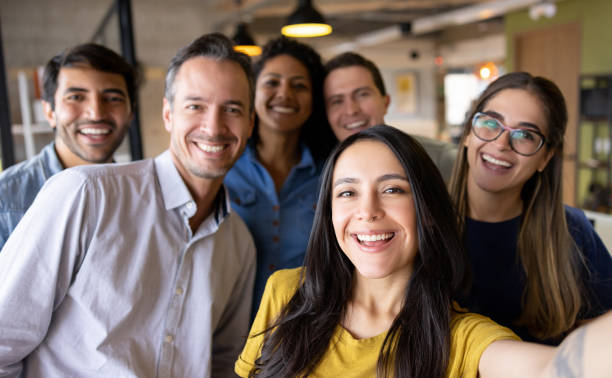
\includegraphics[width=0.75\textwidth,height=7cm,keepaspectratio]{foto-kelompok}\par

		\vspace{0.8cm}
		{\bfseries Disusun oleh:\par}
		\vspace{0.2cm}
		\textbf{Kelompok G04 -- BUMC}
		\vspace{0.5cm} \\
		\begin{tabular}{l l}
			Raynard Fausta & (13524052) \\
			Jason Edward Salim & (13524034) \\
			Athilla Zaidan Zidna Fann & (13524068) \\
		\end{tabular}

		\vfill
		Laboratorium Artificial Intelligence\par
		Program Studi Teknik Informatika\par
		Sekolah Teknik Elektro dan Informatika\par
		Institut Teknologi Bandung\par

	\end{titlepage}

	\clearpage
	\pagestyle{fancy}

	\tableofcontents
	\clearpage
	\listoftables
	\clearpage
	\listoffigures
	\clearpage

	\chapter{Deskripsi Persoalan}
	\section{Latar Belakang}

Mejiro Express ingin menguji coba layanan logistik darat dengan satu truk peti kemas.
Setiap pengiriman perlu mengatur paket mana yang dimuat, di mana paket diletakkan,
dan bagaimana paket diputar agar total nilai (\textit{value}) paket yang terangkut
sebesar mungkin, tanpa melanggar batasan fisik peti kemas. Persoalan ini merupakan
varian persoalan \textit{3D knapsack} / \textit{3D bin packing} yang tergolong NP-hard,
sehingga pencarian solusi eksak tidak praktis untuk ukuran instans yang realistis.
Tugas ini menyelesaikannya dengan algoritma \textit{local search}: Hill-Climbing,
Simulated Annealing, dan Genetic Algorithm~\cite{asisten2026spek}.

\section{Variabel Persoalan}

Setiap paket berbentuk balok dengan atribut berikut.

\begin{table}[H]
	\centering
	\caption{Atribut paket dan truk}
	\label{tab:atribut}
	\begin{tabular}{l l p{8cm}}
		\toprule
		\textbf{Entitas} & \textbf{Atribut} & \textbf{Keterangan} \\
		\midrule
		Paket & \texttt{id} & Identitas paket \\
		& \texttt{w, l, h} & Lebar, panjang, dan tinggi paket \\
		& \texttt{orientation} & Sumbu truk yang sejajar dengan sisi \texttt{w}, \texttt{l}, \texttt{h}; ada enam kemungkinan \\
		& \texttt{value} & Nilai paket \\
		& \texttt{weight} & Berat paket \\
		& \texttt{fragile} & Paket pecah-belah atau tidak \\
		& \texttt{eta} & Perkiraan sisa hari hingga paket harus tiba \\
		\midrule
		Truk & \texttt{w, l, h} & Dimensi peti kemas \\
		& \texttt{max\_capacity} & Berat maksimum yang dapat diangkut \\
		\bottomrule
	\end{tabular}
\end{table}

\section{Fungsi Objektif dan Batasan}

Fungsi objektif yang dimaksimalkan adalah total \textit{value} paket yang berada di
dalam peti kemas:
\begin{equation}
	f(s) = \sum_{i \,:\, \text{paket } i \text{ di dalam truk}} \text{value}_i .
\end{equation}
Paket yang berada di luar truk tidak menyumbang nilai. Sebuah konfigurasi dianggap
valid apabila memenuhi seluruh batasan berikut.

\begin{enumerate}
	\item \textbf{Tidak menembus dinding.} Seluruh bagian paket di dalam truk berada di dalam peti kemas.
	\item \textbf{Tidak saling bertumpuk ruang.} Dua paket tidak boleh menempati ruang yang sama.
	\item \textbf{Tidak melayang.} Paket dengan sudut kiri-bawah-belakang $(x_i,y_i,z_i)$ dan alas
	$B_i=\{(x,y,z_i)\mid x_i\le x<x_i+w_i,\ y_i\le y<y_i+d_i\}$ harus memiliki minimal satu titik
	alas yang ditopang, yaitu $z_i=0$ (lantai truk) atau tepat berada di atas permukaan atas paket lain.
	\item \textbf{Barang pecah-belah tidak menjadi penopang.} Tidak boleh ada paket yang bertumpu di atas paket \textit{fragile}.
	\item \textbf{Kapasitas.} Total berat paket di dalam truk tidak melebihi \texttt{max\_capacity}.
\end{enumerate}

Koordinat berupa bilangan bulat. State awal dibangkitkan secara acak. Aksi tetangga yang
diperbolehkan adalah (1) menukar dua paket, baik di dalam maupun di luar truk,
(2) memindahkan paket ke koordinat lain, dan (3) merotasi paket $90^\circ$ terhadap
sumbu $x$, $y$, atau $z$.

\section{Instans Uji}

Tiga instans dibangkitkan dengan \texttt{src/generate\_instance.py} (\textit{seed} 42) dan
disimpan di \texttt{data/instances/}. Kolom ``batas atas'' adalah nilai optimum
\textit{knapsack} 0/1 dengan batasan berat dan volume yang mengabaikan geometri
(Subbab~\ref{sec:bound}); nilai ini tidak lebih kecil daripada optimum global persoalan.

\begin{table}[H]
	\centering
	\caption{Instans uji}
	\label{tab:instans}
	\begin{tabular}{l c c c c}
		\toprule
		\textbf{Instans} & \textbf{Truk} ($w\times l\times h$) & \textbf{Kapasitas} & \textbf{Jumlah paket} & \textbf{Batas atas} \\
		\midrule
		small  & $6\times8\times5$    & 150  & 15  & 734 \\
		medium & $10\times20\times5$  & 500  & 55  & 2384 \\
		large  & $12\times24\times8$  & 1200 & 120 & 5633 \\
		\bottomrule
	\end{tabular}
\end{table}


	\chapter{Dasar Teori}
	\section{Local Search}

\textit{Local search} bekerja pada satu (atau sekumpulan) \textit{state} lengkap dan
berpindah ke \textit{state} tetangga untuk memperbaiki nilai fungsi objektif. Jalur
pencarian tidak disimpan, sehingga kebutuhan memorinya kecil dan cocok untuk
persoalan optimasi berukuran besar seperti persoalan pengisian peti kemas ini.
Kelemahannya, pencarian dapat terjebak di \textit{local optimum}, \textit{plateau},
atau \textit{ridge}~\cite{russell2010aima,khodra2021localsearch}.

\section{Hill-Climbing}

Hill-Climbing selalu berpindah ke tetangga yang lebih baik dan berhenti ketika tidak
ada tetangga yang lebih baik~\cite{russell2010aima,khodra2021hc}. Varian yang
diimplementasikan:
\begin{itemize}
	\item \textbf{Steepest-ascent}: membangkitkan semua tetangga dan memilih yang terbaik.
	Berhenti bila tetangga terbaik tidak lebih baik daripada \textit{state} sekarang.
	\item \textbf{Stochastic}: memilih secara acak salah satu tetangga yang lebih baik.
	\item \textbf{Sideways move}: seperti \textit{steepest-ascent}, tetapi boleh berpindah ke
	tetangga yang bernilai sama untuk keluar dari \textit{plateau}, dibatasi oleh
	parameter \textit{maximum sideways move}.
	\item \textbf{Random-restart}: menjalankan \textit{steepest-ascent} berulang kali dari
	\textit{state} awal acak yang berbeda dan mengambil hasil terbaik, dibatasi oleh
	parameter \textit{maximum restart}.
\end{itemize}

\section{Simulated Annealing}

Simulated Annealing~\cite{kirkpatrick1983sa,khodra2021sa} memilih satu tetangga acak
setiap iterasi. Tetangga yang lebih baik ($\Delta E>0$) selalu diterima, sedangkan
tetangga yang lebih buruk diterima dengan peluang $e^{\Delta E/T}$. Suhu $T$
diturunkan bertahap sesuai jadwal (\textit{schedule}). Pada suhu tinggi pencarian
bersifat eksploratif, sedangkan pada suhu rendah perilakunya mendekati Hill-Climbing.
Dengan demikian SA dapat keluar dari \textit{local optimum} di awal pencarian.

\section{Genetic Algorithm}

Genetic Algorithm~\cite{russell2010aima,khodra2021ga,kkif2026slides} memelihara
populasi berisi $k$ \textit{state} (individu). Nilai setiap individu diukur dengan
\textit{fitness function}. Generasi berikutnya dibentuk melalui tiga operator:
\begin{enumerate}
	\item \textbf{Seleksi}: induk dipilih dengan peluang sebanding \textit{fitness}
	(\textit{roulette wheel}).
	\item \textbf{Crossover}: dua induk dipotong pada titik acak yang sama, lalu
	bagian ekornya ditukar sehingga terbentuk dua anak.
	\item \textbf{Mutasi}: anak diubah secara acak dengan peluang kecil.
\end{enumerate}


	\chapter{Pembahasan: Implementasi}
	Seluruh program ditulis dalam Python dan berada di folder \texttt{src/}. Bab ini
menjelaskan representasi persoalan, heuristik yang dipakai bersama oleh semua
algoritma, lalu implementasi setiap algoritma. Potongan kode diambil langsung dari
\textit{repository}.

\section{Struktur Program}

\begin{table}[H]
	\centering
	\caption{Modul program}
	\label{tab:modul}
	\begin{tabular}{l p{8.3cm}}
		\toprule
		\textbf{Modul} & \textbf{Isi} \\
		\midrule
		\texttt{core/models.py} & Data statis: \texttt{Package}, \texttt{Truck}, \texttt{Problem} \\
		\texttt{core/validation.py} & Validasi tipe dan rentang parameter serta data instans \\
		\texttt{core/state.py} & Representasi \textit{state}: \texttt{Placement} dan \texttt{State} \\
		\texttt{core/orientation.py} & Enam orientasi paket dan rotasi $90^\circ$ \\
		\texttt{core/geometry.py} & Operasi balok: tumpang tindih, tumpuan, dinding \\
		\texttt{core/constraints.py} & Pendeteksian pelanggaran batasan \\
		\texttt{core/objective.py} & Fungsi objektif \textit{value} dan ETA \\
		\texttt{core/repair.py} & Heuristik \textit{repair} \textit{state} menjadi valid \\
		\texttt{core/neighbors.py} & Aksi \textit{swap}, \textit{move}, \textit{rotate} dan pembangkit tetangga \\
		\texttt{core/initial.py} & \textit{State} awal acak \\
		\texttt{core/bounds.py} & Batas atas optimum global (\textit{knapsack}) \\
		\texttt{core/io.py}, \texttt{core/result.py} & Baca/tulis instans dan hasil \textit{run} (JSON) \\
		\texttt{algorithms/} & Hill-Climbing, Simulated Annealing, Genetic Algorithm \\
		\texttt{experiments/} & Skrip eksperimen HC, SA, dan GA \\
		\texttt{viz/} & Visualisasi 3D \textit{state} dan plot hasil eksperimen \\
		\texttt{main.py} & Antarmuka baris perintah untuk satu kali \textit{run} \\
		\bottomrule
	\end{tabular}
\end{table}

\section{Representasi State}

Data paket dan truk tidak berubah selama pencarian, sehingga dipisahkan dari
\textit{state}. Sebuah \textit{state} adalah \textit{tuple} berisi satu
\texttt{Placement} untuk setiap paket, berurutan sesuai indeks paket. \texttt{Placement}
menyimpan apakah paket berada di dalam truk, koordinat sudut kiri-bawah-belakang
$(x,y,z)$, dan orientasinya. Orientasi ditulis seperti pada spesifikasi, yaitu sumbu
truk yang sejajar dengan sisi \texttt{w}, \texttt{l}, dan \texttt{h}; misalnya
\texttt{("y","x","z")} berarti \{w:y, l:x, h:z\}. Karena semua objek bersifat
\textit{immutable} (\texttt{frozen=True}), \textit{state} dapat langsung dibandingkan
dan disimpan di dalam \textit{set}.

\lstinputlisting[caption={Model persoalan (\texttt{src/core/models.py})},linerange={11-60}]{../src/core/models.py}
\lstinputlisting[caption={Representasi \textit{state} (\texttt{src/core/state.py})}]{../src/core/state.py}

\section{Batasan dan Fungsi Objektif}

\texttt{find\_violations} memeriksa kelima batasan untuk semua paket di dalam truk.
Balok direpresentasikan sebagai interval setengah terbuka $[x_0,x_1)$, sehingga dua
paket yang hanya bersentuhan sisi tidak dianggap bertumpuk. Fungsi
\texttt{rests\_on} mengikuti definisi tumpuan pada spesifikasi: paket atas tepat
berada di permukaan atas paket bawah dan proyeksi alasnya beririsan.

\lstinputlisting[caption={Pemeriksaan batasan (\texttt{src/core/constraints.py})},linerange={16-67}]{../src/core/constraints.py}

Fungsi objektif adalah total \textit{value} paket di dalam truk. Modul ini juga
menyediakan \texttt{evaluate}, yaitu \textit{value} dikurangi penalti sebesar
(\textit{value} paket termahal $+\,1$) untuk setiap pelanggaran. Dengan penalti tersebut,
memasukkan paket secara ilegal tidak pernah lebih menguntungkan daripada
mengeluarkannya. Namun ketiga algoritma pada akhirnya selalu bekerja pada
\textit{state} yang sudah di-\textit{repair} (Subbab~\ref{sec:repair}), sehingga nilai
objektif yang dilaporkan sama dengan total \textit{value} \textit{state} valid.

\lstinputlisting[caption={Fungsi objektif (\texttt{src/core/objective.py})},linerange={24-44}]{../src/core/objective.py}

\section{Heuristik Repair}
\label{sec:repair}

\textit{State} awal acak dan sebagian besar tetangga acak melanggar batasan
(paket melayang atau bertumpuk). Agar pencarian selalu berada di ruang solusi valid,
setiap \textit{state} dilewatkan ke \texttt{repair}. Heuristik ini deterministik dan
hanya \emph{mengeluarkan} atau \emph{menurunkan} paket, tidak pernah menambah paket,
sehingga peningkatan nilai tetap berasal dari algoritma pencarian. Langkahnya:
\begin{enumerate}
	\item Paket yang menembus dinding dikeluarkan dari truk.
	\item Selama total berat melebihi kapasitas, paket dengan rasio
	\textit{value}/berat terendah dikeluarkan.
	\item Paket diproses dari bawah ke atas (urut $z$, lalu \textit{value} terbesar).
	Paket yang bertumpuk dengan paket yang sudah diterima dikeluarkan. Paket lain
	``dijatuhkan'' ke permukaan tertinggi di bawahnya (atau lantai), seperti gravitasi.
	Jika permukaan tempatnya mendarat adalah paket \textit{fragile}, paket dikeluarkan.
\end{enumerate}

\lstinputlisting[caption={Heuristik \textit{repair} untuk satu truk (\texttt{src/core/repair.py})},linerange={38-78}]{../src/core/repair.py}

\section{Aksi Tetangga}

Ketiga aksi pada spesifikasi diimplementasikan sebagai fungsi murni yang
mengembalikan \textit{state} baru:
\texttt{move} memindahkan paket ke koordinat lain atau ke luar truk,
\texttt{rotate} memutar paket $90^\circ$ terhadap suatu sumbu (dua sumbu lainnya
bertukar), dan \texttt{swap} menukar posisi dua paket (masing-masing tetap dengan
orientasinya).

\lstinputlisting[caption={Aksi \textit{move}, \textit{rotate}, dan \textit{swap} (\texttt{src/core/neighbors.py})},linerange={28-54}]{../src/core/neighbors.py}

Ruang koordinat bilangan bulat sangat besar, sedangkan kebanyakan koordinat acak
menghasilkan paket melayang. Karena itu, tujuan aksi \textit{move} diambil dari
\textit{extreme points}~\cite{crainic2008extreme}: titik asal dan titik di kanan,
depan, serta atas setiap paket yang sudah ada di truk, selama paket masih muat di
dalam dinding. Tetangga acak (\texttt{random\_neighbor}) memilih jenis aksi secara
seragam. Untuk \textit{move}, paket di dalam truk dikeluarkan dengan peluang 0,2;
selain itu tujuannya diambil dari \textit{extreme point} (peluang 0,5) atau dari
koordinat acak di dalam dinding. \texttt{all\_neighbors} membangkitkan semua tetangga
untuk \textit{steepest-ascent}: semua rotasi, semua \textit{swap} yang mengubah
sesuatu, serta semua \textit{move} ke luar truk dan ke setiap \textit{extreme point}.

\lstinputlisting[caption={\textit{Extreme points} dan tetangga acak (\texttt{src/core/neighbors.py})},linerange={56-121}]{../src/core/neighbors.py}

\section{State Awal}

Sesuai spesifikasi, \textit{state} awal dibangkitkan acak: setiap paket mendapat
orientasi acak dan, dengan peluang 0,5, dimasukkan ke truk pada koordinat acak di
dalam dinding. \textit{State} ini umumnya tidak valid, lalu di-\textit{repair} oleh
setiap algoritma.

\lstinputlisting[caption={\textit{State} awal acak (\texttt{src/core/initial.py})},linerange={13-32}]{../src/core/initial.py}

\section{Batas Atas Optimum Global}
\label{sec:bound}

Optimum global sebenarnya tidak diketahui. Untuk menilai seberapa dekat hasil setiap
algoritma, dihitung batas atas berupa \textit{knapsack} 0/1 dengan dua batasan, yaitu
berat (kapasitas truk) dan volume (volume peti kemas), yang diselesaikan secara tepat
dengan \textit{dynamic programming}~\cite{martello1990knapsack}. Relaksasi ini
mengabaikan geometri, sehingga nilainya selalu $\ge$ optimum global. Besaran
$\text{gap} = 1 - f(s)/\text{batas atas}$ merupakan batas atas jarak hasil ke optimum
global.

\lstinputlisting[caption={Batas atas \textit{knapsack} (\texttt{src/core/bounds.py})},linerange={14-32}]{../src/core/bounds.py}

\section{Hill-Climbing}

Semua varian Hill-Climbing diimplementasikan di \path{src/algorithms/hill_climbing.py}
(bonus). Setiap tetangga di-\textit{repair} sebelum dinilai. Parameter yang dipakai
pada eksperimen: \texttt{max\_iterations}=100, \texttt{neighbor\_samples}=50 untuk
\textit{stochastic}, \texttt{max\_sideways}=20, dan \texttt{max\_restarts}=5 (instans
\textit{large} memakai 2 karena waktu eksekusinya lama).

\begin{itemize}
	\item \textbf{Steepest-ascent} memakai \texttt{\_best\_neighbor}, yang menilai seluruh
	\texttt{all\_neighbors}. Berhenti jika tetangga terbaik tidak lebih baik.
	\item \textbf{Stochastic} memilih secara acak salah satu tetangga yang lebih baik.
	Untuk menghemat waktu, mula-mula diambil 50 tetangga acak. Jika tidak ada yang lebih
	baik, seluruh \texttt{all\_neighbors} diperiksa dan salah satu tetangga yang lebih baik
	dipilih secara seragam. Pencarian berhenti hanya jika tidak ada satu pun tetangga yang
	lebih baik (\textit{local optimum}) atau \texttt{max\_iterations} tercapai.
	\item \textbf{Sideways move} seperti \textit{steepest-ascent}, tetapi boleh pindah ke
	tetangga bernilai sama yang belum pernah dikunjungi. Berhenti ketika banyak
	\textit{sideways move} mencapai \texttt{max\_sideways}. Karena tetangga bernilai sama
	yang sudah dikunjungi tidak dipilih lagi, pencarian tidak dapat berputar dalam siklus.
	\item \textbf{Random-restart} menjalankan \textit{steepest-ascent} dari \textit{state}
	awal acak sebanyak \texttt{max\_restarts}$+1$ kali dan mengambil hasil terbaik.
	Banyak iterasi per \textit{restart} dicatat.
\end{itemize}

\lstinputlisting[caption={Satu kali pendakian Hill-Climbing (\texttt{src/algorithms/hill\_climbing.py})},linerange={109-171}]{../src/algorithms/hill_climbing.py}

\section{Simulated Annealing}

Simulated Annealing diimplementasikan di \path{src/algorithms/simulated_annealing.py}.
Setiap iterasi mengambil satu tetangga acak yang sudah di-\textit{repair}. Tetangga
diterima jika $\Delta E\ge 0$; jika tidak, diterima dengan peluang $e^{\Delta E/T}$.
Heuristik yang dipakai:
\begin{itemize}
	\item \textbf{Kalibrasi suhu awal.} Jika $T_0$ tidak diberikan, diambil 100 tetangga
	acak dari \textit{state} awal dan dihitung rata-rata $|\Delta E|$ langkah yang
	memburuk, lalu $T_0=-\overline{|\Delta E|}/\ln p_0$. Dengan begitu, langkah memburuk
	rata-rata diterima dengan peluang $p_0$ di awal pencarian~\cite{benameur2004t0}.
	\item \textbf{Jadwal dengan titik ujung tetap.} Iterasi pertama memakai $T_0$ dan iterasi
	terakhir tepat $T_{\min}$, secara geometrik ($T_k=T_0(T_{\min}/T_0)^{k/(n-1)}$,
	$k=0,\dots,n-1$) atau linear.
	Banyak iterasi menjadi satu-satunya parameter biaya.
	\item \textbf{Simpan \textit{state} terbaik.} Hasil akhir adalah \textit{state} terbaik
	yang pernah dikunjungi, bukan \textit{state} terakhir.
	\item \textbf{Ratio swap (opsional).} Dengan peluang \texttt{ratio\_bias}, tetangga yang
	diusulkan adalah \textit{swap} antara paket di dalam truk yang rasio
	\textit{value}/beratnya rendah dan paket di luar yang rasionya tinggi. Aksinya
	tetap \textit{swap} biasa; hanya pemilihan paketnya yang dibias.
	\item \textbf{Definisi \textit{stuck}.} SA dianggap \textit{stuck} di \textit{local optimum}
	jika nilai objektif \textit{state} sekarang tidak berubah selama 500 iterasi
	berturut-turut. Satu \textit{plateau} dihitung satu kali.
\end{itemize}

\lstinputlisting[caption={Kalibrasi $T_0$, jadwal suhu, dan peluang penerimaan (\texttt{src/algorithms/simulated\_annealing.py})},linerange={48-66,94-106}]{../src/algorithms/simulated_annealing.py}
\lstinputlisting[caption={Iterasi utama Simulated Annealing (\texttt{src/algorithms/simulated\_annealing.py})},linerange={110-189}]{../src/algorithms/simulated_annealing.py}

\section{Genetic Algorithm}
\label{sec:ga-impl}

Genetic Algorithm diimplementasikan di \path{src/algorithms/genetic.py} mengikuti
salindia kuliah~\cite{kkif2026slides}:
\begin{itemize}
	\item \textbf{Individu} adalah satu \textit{state} lengkap; gen ke-$i$ adalah
	\texttt{Placement} paket ke-$i$.
	\item \textbf{Populasi awal} berisi $k$ \textit{state} acak yang di-\textit{repair}.
	\item \textbf{Fitness} adalah total \textit{value} (fungsi objektif).
	\item \textbf{Seleksi} memakai \textit{roulette wheel} (\texttt{roulette\_select}).
	\item \textbf{Crossover} memakai \textit{single-point crossover}: titik potong acak di
	$[1,n-1]$, kedua induk bertukar ekor sehingga terbentuk dua anak.
	\item \textbf{Mutasi}: dengan peluang 0,2, anak dikenai satu aksi tetangga acak
	(\textit{move}/\textit{rotate}/\textit{swap}).
\end{itemize}
Ada tiga adaptasi terhadap versi salindia. Pertama, setiap anak di-\textit{repair},
karena hasil \textit{crossover} dapat bertumpuk atau melayang. Kedua, satu individu
terbaik dibawa langsung ke generasi berikutnya (\textit{elitism}). Ketiga, mutasi
memakai aksi tetangga, bukan mengganti satu karakter \textit{string}, karena gen
berisi posisi dan orientasi paket.

\lstinputlisting[caption={Seleksi dan \textit{crossover} (\texttt{src/algorithms/genetic.py})},linerange={34-49}]{../src/algorithms/genetic.py}
\lstinputlisting[caption={Iterasi utama Genetic Algorithm (\texttt{src/algorithms/genetic.py})},linerange={52-101}]{../src/algorithms/genetic.py}

\section{Bonus: Fungsi Objektif Berbasis ETA}

Sebagai fungsi objektif alternatif tanpa menambah variabel, \textit{value} setiap
paket dibagi dengan ETA-nya:
\begin{equation}
	f_{\text{ETA}}(s)=\sum_{i \,:\, \text{paket } i \text{ di dalam truk}} \frac{\text{value}_i}{\text{ETA}_i}.
\end{equation}
Paket yang harus tiba lebih cepat (ETA kecil) menjadi lebih berharga, sehingga
truk memprioritaskan paket yang mendesak. Objektif ini dipilih dengan opsi
\texttt{--objective eta} dan berlaku untuk ketiga algoritma.

\section{Bonus: Multi-Truk}
\label{sec:multitruck-impl}

Program dapat menerima armada berisi $N$ truk identik (opsi \texttt{--trucks N} atau
\texttt{"truck\_count"} pada JSON instans). Setiap truk memakai dimensi dan kapasitas
\texttt{truck} dari instans. Objektifnya adalah total \textit{value} paket yang
diangkut seluruh armada, dan setiap paket hanya dapat berada di satu truk.
Perubahan utamanya:
\begin{itemize}
	\item \textbf{Representasi.} \texttt{Placement} mendapat atribut \texttt{truck\_id};
	\texttt{Problem} mendapat \texttt{truck\_count}.
	\item \textbf{Batasan dan \textit{repair}} dijalankan terpisah untuk setiap truk.
	Dinding, tumpang tindih, tumpuan, \textit{fragile}, dan kapasitas berat hanya
	membandingkan paket di truk yang sama. Paket dengan \texttt{truck\_id} tidak valid
	dikeluarkan.
	\item \textbf{Aksi tetangga.} \textit{Move} dapat memindahkan paket ke truk lain
	(tujuannya \textit{extreme point} di truk tujuan), dan \textit{swap} menukar posisi
	sekaligus truk dua paket. \texttt{all\_neighbors} membangkitkan \textit{move} ke
	setiap truk. Ketiga algoritma tidak perlu diubah karena bekerja melalui operator
	yang sama.
	\item \textbf{Batas atas} memakai kapasitas berat dan volume gabungan armada,
	tetap sebagai relaksasi \textit{knapsack}.
	\item \textbf{Visualisasi} menampilkan setiap truk beserta berat muatannya.
\end{itemize}
Untuk satu truk, urutan bilangan acak yang dipakai tidak berubah, sehingga seluruh
hasil eksperimen satu truk tetap dapat direproduksi persis.

\lstinputlisting[caption={\textit{Repair} per truk (\texttt{src/core/repair.py})},linerange={23-35}]{../src/core/repair.py}

\section{Visualisasi dan Keluaran}

Setiap \textit{run} menyimpan satu folder di \texttt{output/} berisi
\texttt{result.json} (parameter, \textit{seed}, durasi, \textit{state} awal dan akhir,
riwayat nilai), \texttt{initial.png} dan \texttt{final.png} (visualisasi 3D
\textit{state}), serta \texttt{curve.png} (plot objektif terhadap iterasi). Untuk SA
ada tambahan \texttt{eet.png} (plot $e^{\Delta E/T}$). Visualisasi 3D menampilkan isi
peti kemas (paket \textit{fragile} bertepi merah), nilai \textit{state}, total berat,
dan daftar paket di luar truk (Gambar~\ref{fig:render}). Skrip eksperimen juga
menyimpan \texttt{summary.csv} dan plot pembanding.

\begin{figure}[H]
	\centering
	\begin{subfigure}{0.49\textwidth}
		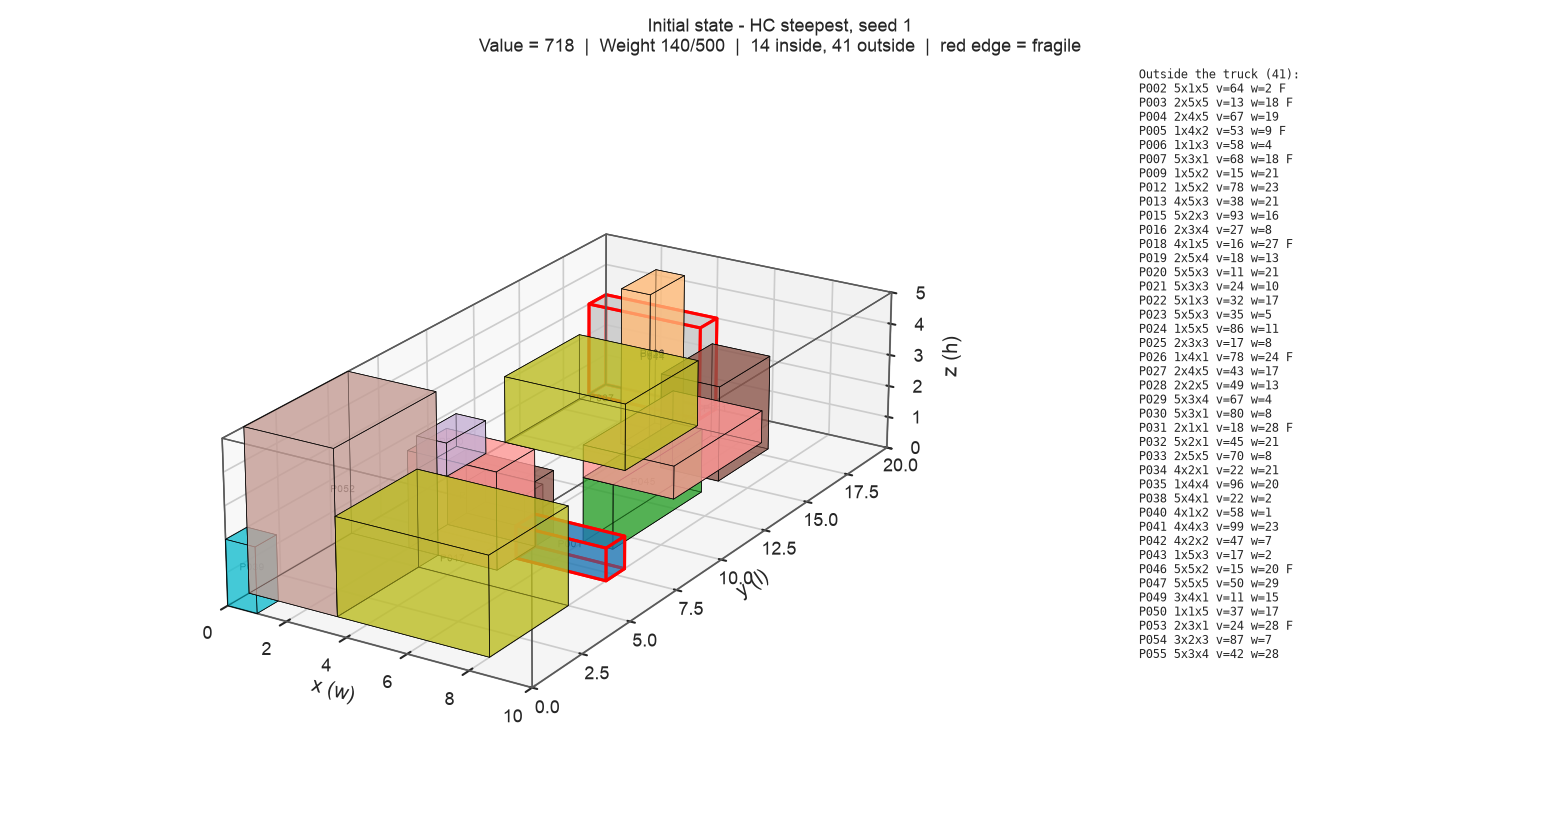
\includegraphics[width=\textwidth]{hc/medium/steepest/seed1/initial.png}
		\caption{\textit{State} awal}
	\end{subfigure}
	\begin{subfigure}{0.49\textwidth}
		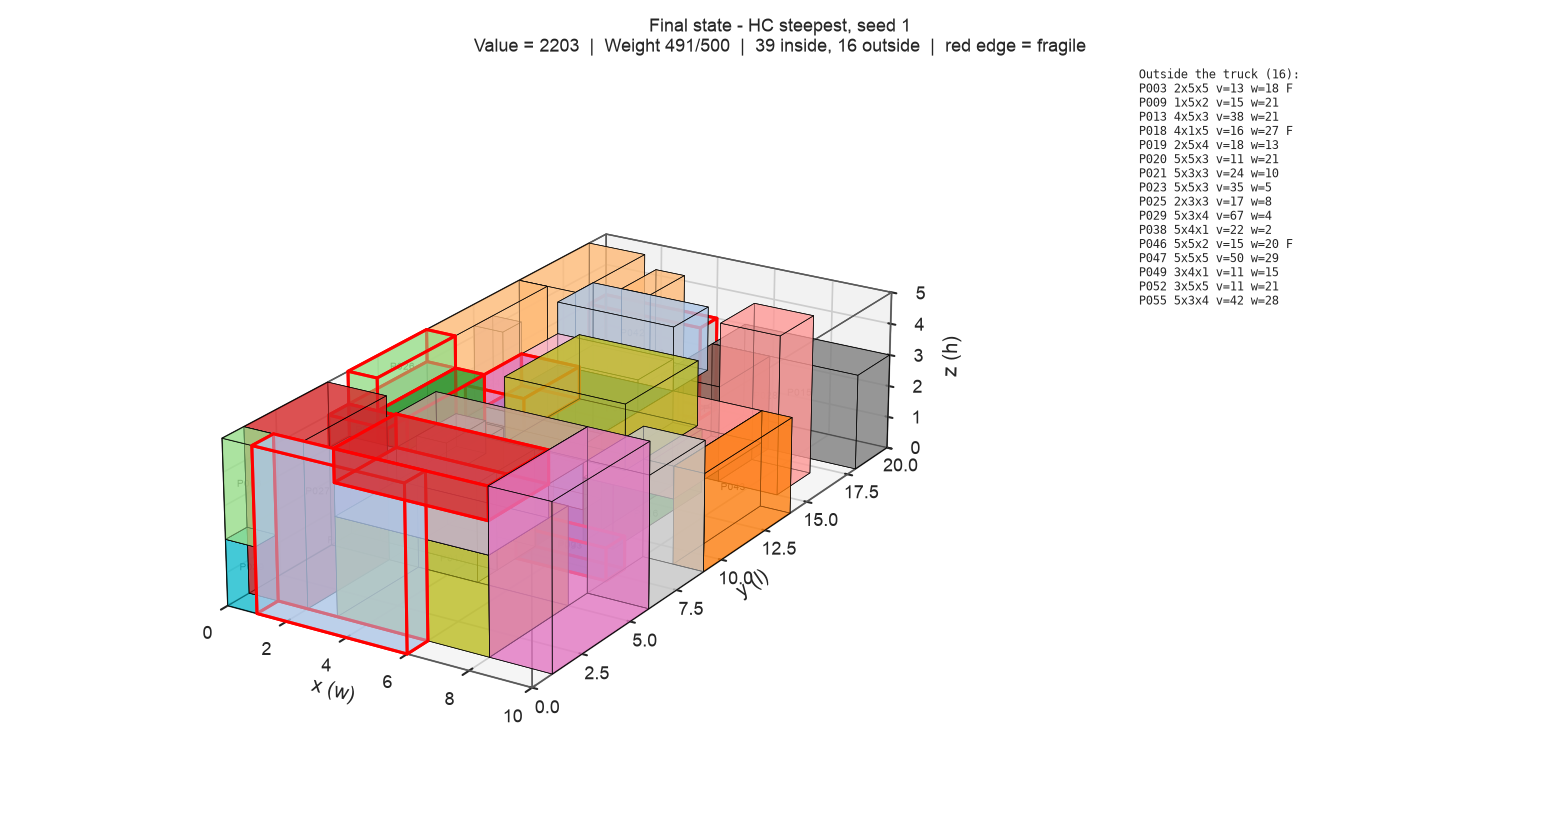
\includegraphics[width=\textwidth]{hc/medium/steepest/seed1/final.png}
		\caption{\textit{State} akhir}
	\end{subfigure}
	\caption{Visualisasi \textit{state} awal dan akhir (HC \textit{steepest-ascent}, instans \textit{medium}, \textit{seed} 1)}
	\label{fig:render}
\end{figure}

Program dijalankan melalui \texttt{src/main.py} untuk satu kali \textit{run}, misalnya:
\begin{lstlisting}[language=bash]
python -m src.main hc --instance data/instances/medium.json --variant steepest --seed 1
python -m src.main sa --instance data/instances/medium.json --iters 20000 --p0 0.01
python -m src.main ga --instance data/instances/medium.json --pop 50 --gens 100
\end{lstlisting}
Eksperimen lengkap dijalankan dengan modul \texttt{src.experiments.hc\_experiment}, \texttt{sa\_experiment}, dan \texttt{ga\_experiment}.


	\chapter{Pembahasan: Hasil dan Analisis Eksperimen}
	\section{Metodologi Eksperimen}

Setiap konfigurasi dijalankan 3 kali (\textit{seed} 1, 2, 3) pada ketiga instans.
Setiap pasangan (konfigurasi, \textit{seed}) mendapat \textit{seed} acak tersendiri yang
diturunkan dari nama konfigurasinya (\texttt{run\_seed}). Dengan demikian, misalnya,
GA 50 generasi bukan potongan awal dari GA 200 generasi, dan setiap \textit{run}
dapat direproduksi persis. Durasi diukur dengan \texttt{time.perf\_counter} untuk satu
\textit{run} dalam satu proses Python. Seluruh angka pada bab ini diambil dari
\texttt{output/*/*/summary.csv}. Folder setiap \textit{run} berisi \textit{state} awal
dan akhir (JSON dan gambar 3D) serta plot objektif terhadap iterasi.

Kolom \textbf{gap} adalah $1-f(s)/\text{batas atas}$ (Subbab~\ref{sec:bound}), yaitu
batas atas jarak hasil ke optimum global. Gap 0\% berarti hasilnya terbukti optimum global.

\section{Hasil Hill-Climbing}

Tabel~\ref{tab:hc-summary} merangkum keempat varian. Hasil setiap \textit{run}, termasuk
banyak iterasi, alasan berhenti, serta banyak \textit{restart} dan iterasi per
\textit{restart}, ada pada Tabel~\ref{tab:hc-runs}.

\begin{table}[H]\centering\small
\caption{Ringkasan Hill-Climbing (rata-rata 3 \textit{run})}\label{tab:hc-summary}
\begin{adjustbox}{max width=\textwidth}\begin{tabular}{l l r r r r r}
\toprule
\textbf{Instans} & \textbf{Varian} & \textbf{Akhir (mean $\pm$ std)} & \textbf{Min--maks} & \textbf{Gap (\%)} & \textbf{Durasi (s)} & \textbf{Iterasi} \\
\midrule
\multirow{4}{*}{\textit{small}} & Steepest & 680.7 $\pm$ 24.4 & 661--708 & 7.3 & 0.29 & 8.3 \\
 & Stochastic & 538.3 $\pm$ 115.0 & 406--614 & 26.7 & 0.03 & 7.0 \\
 & Sideways & 682.0 $\pm$ 45.0 & 630--708 & 7.1 & 1.18 & 28.7 \\
 & Random-restart & 712.7 $\pm$ 8.1 & 708--722 & 2.9 & 1.21 & 40.7 \\
\midrule
\multirow{4}{*}{\textit{medium}} & Steepest & 2213.7 $\pm$ 23.9 & 2197--2241 & 7.1 & 53.51 & 29.3 \\
 & Stochastic & 1469.7 $\pm$ 58.4 & 1404--1516 & 38.4 & 0.29 & 23.7 \\
 & Sideways & 2192.7 $\pm$ 12.7 & 2178--2201 & 8.0 & 50.77 & 47.7 \\
 & Random-restart & 2260.7 $\pm$ 7.2 & 2256--2269 & 5.2 & 120.72 & 167.7 \\
\midrule
\multirow{4}{*}{\textit{large}} & Steepest & 5205.7 $\pm$ 21.6 & 5181--5221 & 7.6 & 693.51 & 64.0 \\
 & Stochastic & 3061.0 $\pm$ 163.6 & 2912--3236 & 45.7 & 0.81 & 41.0 \\
 & Sideways & 5179.7 $\pm$ 91.9 & 5107--5283 & 8.0 & 922.48 & 82.3 \\
 & Random-restart & 5261.7 $\pm$ 46.1 & 5209--5295 & 6.6 & 1683.70 & 186.3 \\
\bottomrule
\end{tabular}\end{adjustbox}
\end{table}


\begin{figure}[H]
	\centering
	\begin{subfigure}{0.49\textwidth}
		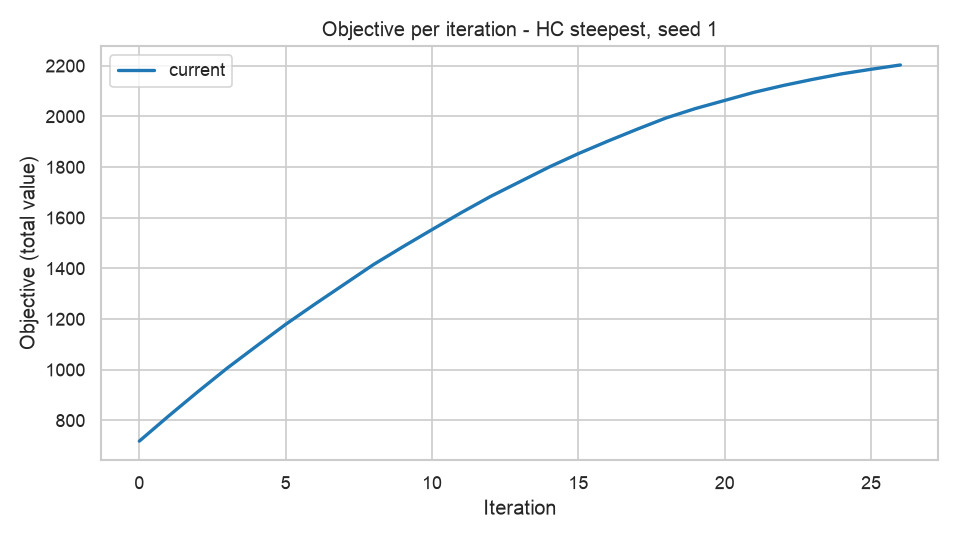
\includegraphics[width=\textwidth]{hc/medium/steepest/seed1/curve.png}
		\caption{\textit{Steepest-ascent}}
	\end{subfigure}
	\begin{subfigure}{0.49\textwidth}
		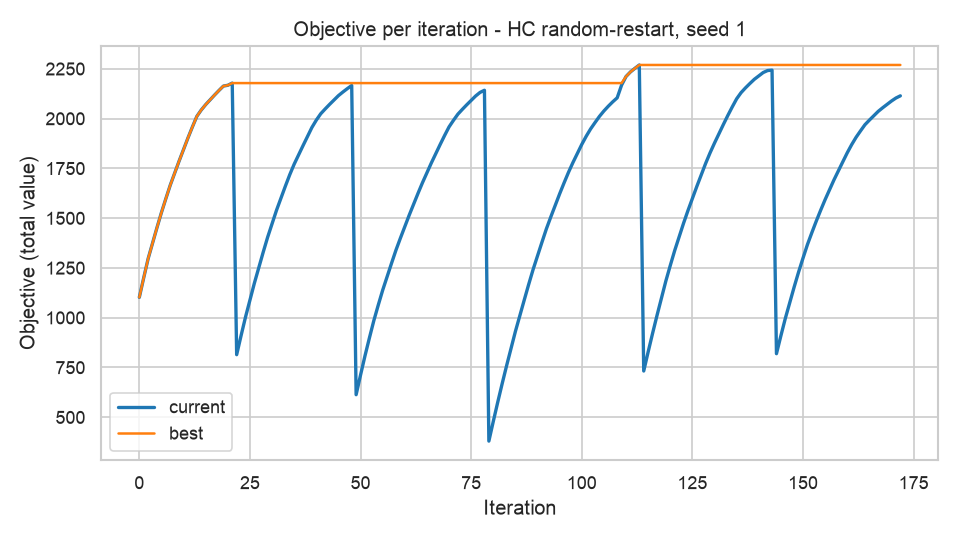
\includegraphics[width=\textwidth]{hc/medium/random-restart/seed1/curve.png}
		\caption{\textit{Random-restart}}
	\end{subfigure}
	\caption{Nilai objektif terhadap iterasi Hill-Climbing (instans \textit{medium}, \textit{seed} 1)}
	\label{fig:hc-curve}
\end{figure}

\begin{figure}[H]
	\centering
	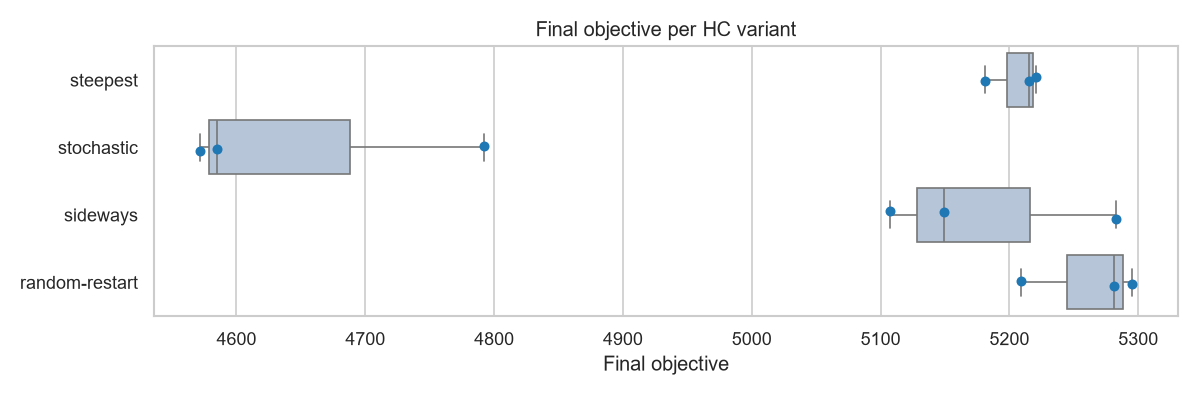
\includegraphics[width=0.75\textwidth]{hc/large/final_value_box.png}
	\caption{Sebaran nilai akhir varian Hill-Climbing (instans \textit{large})}
	\label{fig:hc-box}
\end{figure}

{\scriptsize\setlength{\tabcolsep}{4pt}
\begin{longtable}{l c r r r r r p{3.6cm}}
\caption{Hasil setiap \textit{run} Hill-Climbing}\label{tab:hc-runs}\\
\toprule
\textbf{Varian} & \textbf{Seed} & \textbf{Awal} & \textbf{Akhir} & \textbf{Gap (\%)} & \textbf{Durasi (s)} & \textbf{Iterasi} & \textbf{Berhenti karena} \\
\endfirsthead
\toprule
\textbf{Varian} & \textbf{Seed} & \textbf{Awal} & \textbf{Akhir} & \textbf{Gap (\%)} & \textbf{Durasi (s)} & \textbf{Iterasi} & \textbf{Berhenti karena} \\
\endhead
\midrule
\multicolumn{8}{l}{\textit{small} (batas atas 734)} \\
Steepest & 1 & 119 & 708 & 3.5 & 0.17 & 11 & local optimum \\
Steepest & 2 & 222 & 661 & 10.0 & 0.20 & 7 & local optimum \\
Steepest & 3 & 209 & 673 & 8.3 & 0.49 & 7 & local optimum \\
Stochastic & 1 & 270 & 615 & 16.2 & 0.10 & 10 & local optimum \\
Stochastic & 2 & 347 & 708 & 3.5 & 0.09 & 13 & local optimum \\
Stochastic & 3 & 317 & 708 & 3.5 & 0.10 & 10 & local optimum \\
Sideways & 1 & 235 & 630 & 14.2 & 1.27 & 27 & max sideways \\
Sideways & 2 & 189 & 708 & 3.5 & 1.20 & 29 & max sideways \\
Sideways & 3 & 279 & 708 & 3.5 & 1.07 & 30 & max sideways \\
Random-restart & 1 & 434 & 708 & 3.5 & 0.99 & 37 & max restart (5 restart: 4, 8, 7, 7, 5, 6) \\
Random-restart & 2 & 151 & 722 & 1.6 & 1.28 & 46 & max restart (5 restart: 8, 6, 9, 4, 10, 9) \\
Random-restart & 3 & 212 & 708 & 3.5 & 1.36 & 39 & max restart (5 restart: 8, 7, 6, 3, 7, 8) \\
\midrule
\multicolumn{8}{l}{\textit{medium} (batas atas 2384)} \\
Steepest & 1 & 718 & 2203 & 7.6 & 49.65 & 26 & local optimum \\
Steepest & 2 & 532 & 2197 & 7.8 & 86.02 & 31 & local optimum \\
Steepest & 3 & 602 & 2241 & 6.0 & 24.84 & 31 & local optimum \\
Stochastic & 1 & 944 & 2132 & 10.6 & 17.81 & 36 & local optimum \\
Stochastic & 2 & 361 & 2144 & 10.1 & 23.74 & 62 & local optimum \\
Stochastic & 3 & 674 & 2040 & 14.4 & 16.71 & 46 & local optimum \\
Sideways & 1 & 704 & 2199 & 7.8 & 49.59 & 47 & max sideways \\
Sideways & 2 & 732 & 2201 & 7.7 & 50.30 & 48 & max sideways \\
Sideways & 3 & 658 & 2178 & 8.6 & 52.40 & 48 & max sideways \\
Random-restart & 1 & 1102 & 2269 & 4.8 & 126.60 & 167 & max restart (5 restart: 21, 26, 29, 34, 29, 28) \\
Random-restart & 2 & 702 & 2256 & 5.4 & 117.72 & 163 & max restart (5 restart: 30, 29, 30, 23, 27, 24) \\
Random-restart & 3 & 794 & 2257 & 5.3 & 117.85 & 173 & max restart (5 restart: 28, 31, 27, 33, 28, 26) \\
\midrule
\multicolumn{8}{l}{\textit{large} (batas atas 5633)} \\
Steepest & 1 & 1485 & 5221 & 7.3 & 878.74 & 65 & local optimum \\
Steepest & 2 & 1379 & 5181 & 8.0 & 579.39 & 64 & local optimum \\
Steepest & 3 & 1506 & 5215 & 7.4 & 622.42 & 63 & local optimum \\
Stochastic & 1 & 1443 & 4585 & 18.6 & 441.50 & 100 & max iterasi \\
Stochastic & 2 & 1668 & 4792 & 14.9 & 800.63 & 96 & local optimum \\
Stochastic & 3 & 1475 & 4572 & 18.8 & 560.71 & 100 & max iterasi \\
Sideways & 1 & 1644 & 5107 & 9.3 & 934.22 & 82 & max sideways \\
Sideways & 2 & 1584 & 5283 & 6.2 & 838.40 & 81 & max sideways \\
Sideways & 3 & 1689 & 5149 & 8.6 & 994.83 & 84 & max sideways \\
Random-restart & 1 & 1989 & 5281 & 6.2 & 1654.99 & 185 & max restart (2 restart: 52, 67, 66) \\
Random-restart & 2 & 1329 & 5295 & 6.0 & 1698.62 & 189 & max restart (2 restart: 65, 59, 65) \\
Random-restart & 3 & 1586 & 5209 & 7.5 & 1697.51 & 185 & max restart (2 restart: 61, 61, 63) \\
\bottomrule
\end{longtable}
}


\section{Hasil Simulated Annealing}

Konfigurasi utama SA memakai jadwal geometrik, 20.000 iterasi, $p_0=0{,}01$, dan
$T_{\min}=0{,}05$ (Tabel~\ref{tab:sa-runs}). Gambar~\ref{fig:sa-curve} menunjukkan
plot objektif dan $e^{\Delta E/T}$ terhadap iterasi. Kolom \textbf{Stuck} adalah
frekuensi SA \textit{stuck} di \textit{local optimum}, yaitu banyaknya \textit{plateau}
dengan nilai objektif tidak berubah selama minimal 500 iterasi.

\begin{table}[H]\centering\small
\caption{Hasil setiap \textit{run} Simulated Annealing (geometrik, 20.000 iterasi, $p_0=0{,}01$, $T_{\min}=0{,}05$)}\label{tab:sa-runs}
\begin{adjustbox}{max width=\textwidth}\begin{tabular}{c r r r r r r r}
\toprule
\textbf{Seed} & \textbf{Awal} & \textbf{Akhir} & \textbf{Gap (\%)} & \textbf{Durasi (s)} & \textbf{$T_0$} & \textbf{Stuck} & \textbf{Iterasi terbaik} \\
\midrule
\multicolumn{8}{l}{\textit{small} (batas atas 734)} \\
1 & 244 & 734 & 0.0 & 4.62 & 9.28 & 4 & 11860 \\
2 & 94 & 734 & 0.0 & 4.75 & 9.19 & 1 & 776 \\
3 & 289 & 734 & 0.0 & 4.53 & 15.12 & 3 & 8718 \\
\midrule
\multicolumn{8}{l}{\textit{medium} (batas atas 2384)} \\
1 & 899 & 2248 & 5.7 & 23.12 & 12.47 & 4 & 12907 \\
2 & 710 & 2209 & 7.3 & 23.24 & 12.08 & 7 & 19857 \\
3 & 639 & 2243 & 5.9 & 22.75 & 9.83 & 8 & 15616 \\
\midrule
\multicolumn{8}{l}{\textit{large} (batas atas 5633)} \\
1 & 1669 & 4932 & 12.4 & 21.09 & 11.17 & 7 & 18777 \\
2 & 1505 & 4943 & 12.2 & 21.87 & 8.11 & 11 & 18974 \\
3 & 1433 & 5053 & 10.3 & 21.56 & 9.66 & 7 & 16325 \\
\bottomrule
\end{tabular}\end{adjustbox}
\end{table}


\begin{figure}[H]
	\centering
	\begin{subfigure}{0.49\textwidth}
		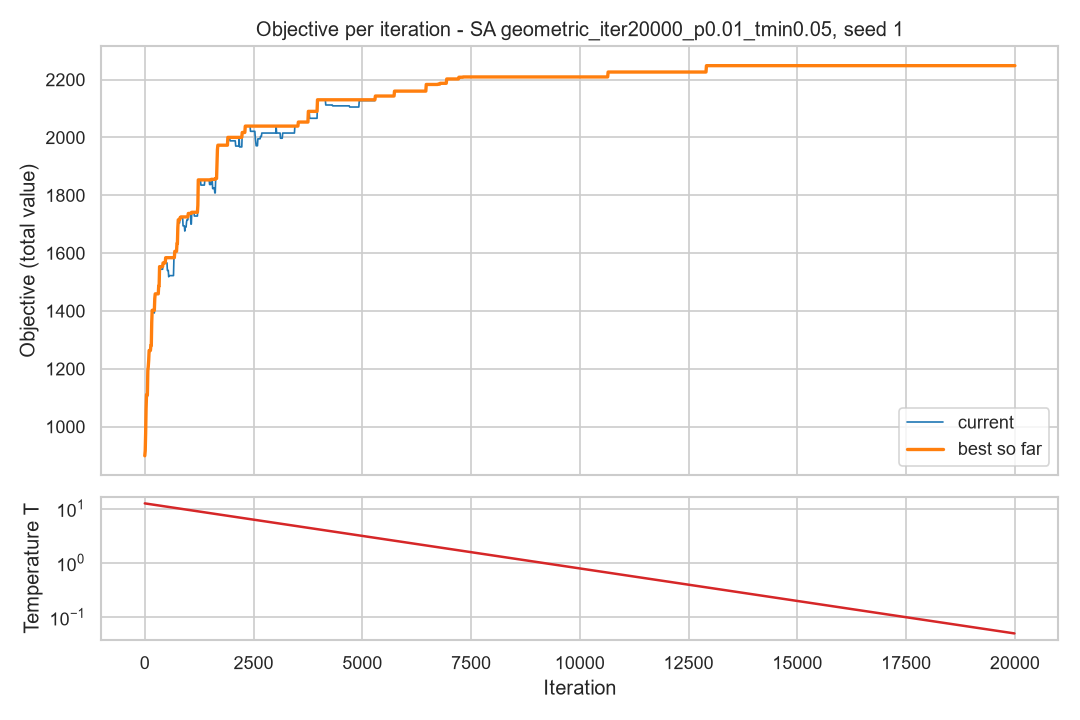
\includegraphics[width=\textwidth]{sa/medium/geometric_iter20000_p0.01_tmin0.05/seed1/curve.png}
		\caption{Nilai objektif dan suhu}
	\end{subfigure}
	\begin{subfigure}{0.49\textwidth}
		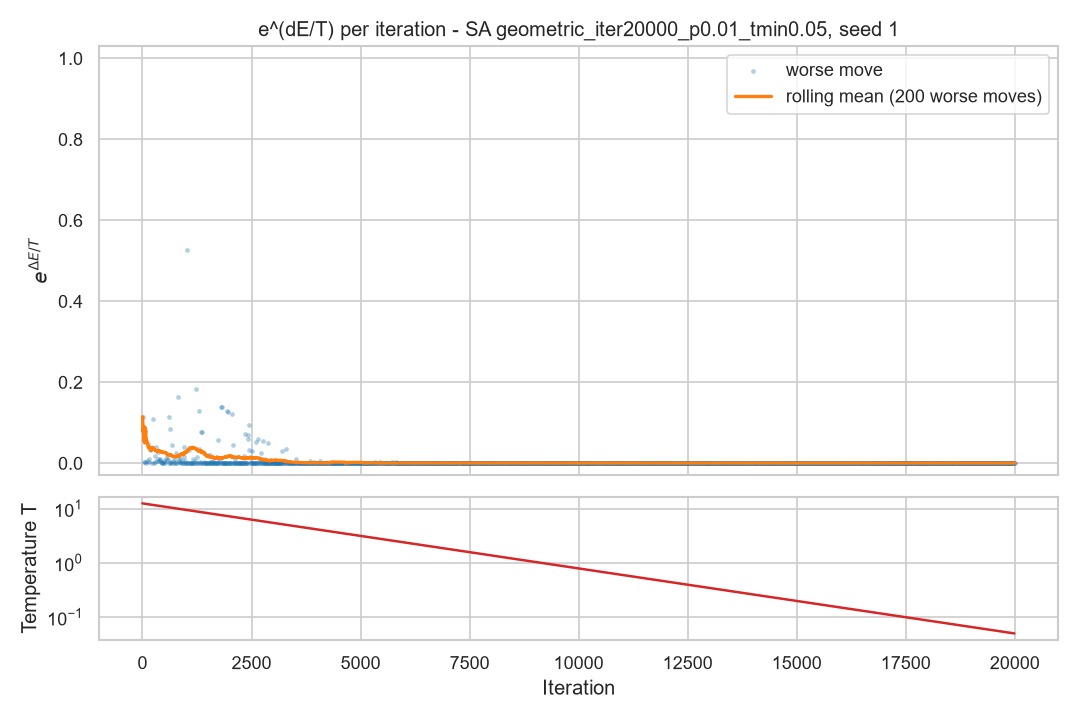
\includegraphics[width=\textwidth]{sa/medium/geometric_iter20000_p0.01_tmin0.05/seed1/eet.png}
		\caption{$e^{\Delta E/T}$}
	\end{subfigure}
	\caption{Simulated Annealing pada instans \textit{medium} (\textit{seed} 1)}
	\label{fig:sa-curve}
\end{figure}

Parameter SA juga diuji pada instans \textit{medium}, satu parameter divariasikan
setiap kali (Tabel~\ref{tab:sa-params}, Gambar~\ref{fig:sa-compare}).

\begin{table}[H]\centering\scriptsize
\caption{Pengaruh parameter Simulated Annealing pada instans \textit{medium} (rata-rata 3 \textit{run})}\label{tab:sa-params}
\begin{adjustbox}{max width=\textwidth}\begin{tabular}{l l r r r r r r r r}
\toprule
\textbf{Variasi} & \textbf{Jadwal} & \textbf{Iterasi} & \textbf{$p_0$} & \textbf{$T_{\min}$} & \textbf{Bias} & \textbf{Akhir} & \textbf{Gap (\%)} & \textbf{Durasi (s)} & \textbf{Stuck} \\
\midrule
\multirow{5}{*}{Iterasi} & geometric & 2500 & 0.8 & 0.05 & 0 & 1985.7 $\pm$ 41.5 & 16.7 & 1.7 & 0.0 \\
 & geometric & 5000 & 0.8 & 0.05 & 0 & 2075.7 $\pm$ 14.7 & 12.9 & 3.8 & 1.3 \\
 & geometric & 10000 & 0.8 & 0.05 & 0 & 2187.7 $\pm$ 49.0 & 8.2 & 8.4 & 2.7 \\
 & geometric & 20000 & 0.8 & 0.05 & 0 & 2226.0 $\pm$ 30.0 & 6.6 & 16.8 & 5.7 \\
 & geometric & 40000 & 0.8 & 0.05 & 0 & 2262.3 $\pm$ 13.2 & 5.1 & 37.3 & 10.0 \\
\midrule
\multirow{5}{*}{$p_0$} & geometric & 10000 & 0.01 & 0.05 & 0 & 2232.3 $\pm$ 18.6 & 6.4 & 10.7 & 5.0 \\
 & geometric & 10000 & 0.2 & 0.05 & 0 & 2163.3 $\pm$ 37.3 & 9.3 & 10.1 & 3.3 \\
 & geometric & 10000 & 0.5 & 0.05 & 0 & 2169.3 $\pm$ 39.1 & 9.0 & 8.9 & 3.3 \\
 & geometric & 10000 & 0.8 & 0.05 & 0 & 2187.7 $\pm$ 49.0 & 8.2 & 8.4 & 2.7 \\
 & geometric & 10000 & 0.95 & 0.05 & 0 & 2147.0 $\pm$ 13.5 & 9.9 & 7.6 & 2.3 \\
\midrule
\multirow{2}{*}{Jadwal} & geometric & 10000 & 0.8 & 0.05 & 0 & 2187.7 $\pm$ 49.0 & 8.2 & 8.4 & 2.7 \\
 & linear & 10000 & 0.8 & 0.05 & 0 & 1755.7 $\pm$ 69.0 & 26.4 & 3.3 & 0.0 \\
\midrule
\multirow{4}{*}{$T_{\min}$} & geometric & 10000 & 0.8 & 0.05 & 0 & 2187.7 $\pm$ 49.0 & 8.2 & 8.4 & 2.7 \\
 & geometric & 10000 & 0.8 & 0.5 & 0 & 2149.0 $\pm$ 79.1 & 9.9 & 8.0 & 2.7 \\
 & geometric & 10000 & 0.8 & 2 & 0 & 2132.3 $\pm$ 64.6 & 10.6 & 6.9 & 0.3 \\
 & geometric & 10000 & 0.8 & 5 & 0 & 1994.3 $\pm$ 17.2 & 16.3 & 5.6 & 0.3 \\
\midrule
\multirow{3}{*}{Ratio bias} & geometric & 20000 & 0.01 & 0.05 & 0 & 2233.3 $\pm$ 21.2 & 6.3 & 23.0 & 6.3 \\
 & geometric & 20000 & 0.01 & 0.05 & 0.2 & 2247.3 $\pm$ 35.0 & 5.7 & 22.4 & 5.7 \\
 & geometric & 20000 & 0.01 & 0.05 & 0.5 & 2251.7 $\pm$ 40.4 & 5.5 & 241.7 & 5.3 \\
\bottomrule
\end{tabular}\end{adjustbox}
\end{table}


Rata-rata durasi \textit{ratio bias} 0,5 pada Tabel~\ref{tab:sa-params} dipengaruhi satu
\textit{run} (\textit{seed} 1) yang tercatat 683 detik, padahal dua \textit{run} lainnya
sekitar 21 detik. Nilai objektifnya tidak terpengaruh.

\begin{figure}[H]
	\centering
	\begin{subfigure}{0.49\textwidth}
		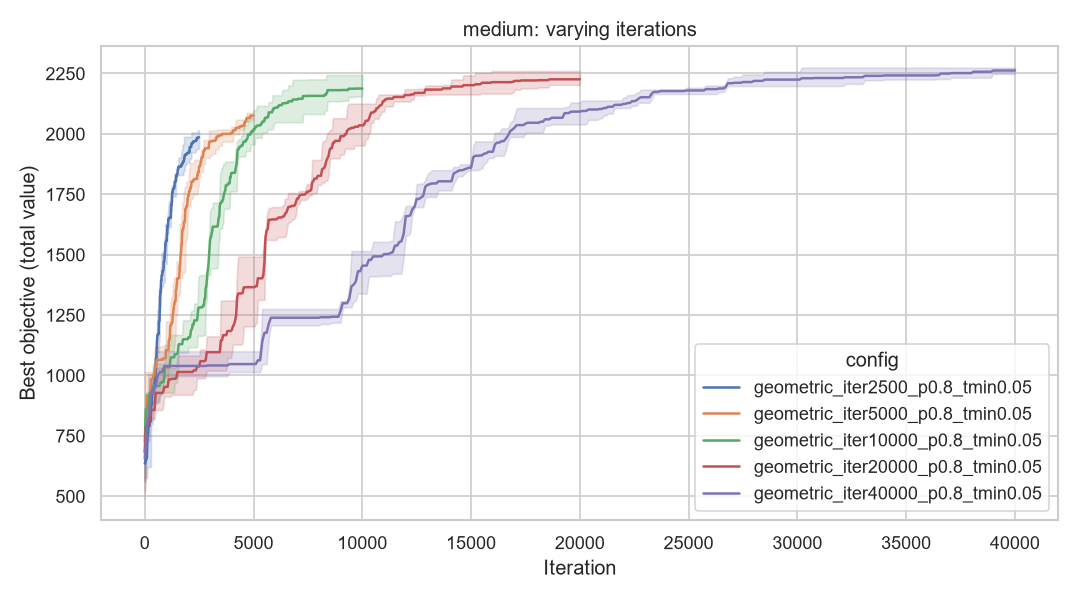
\includegraphics[width=\textwidth]{sa/medium/compare_iterations.png}
		\caption{Banyak iterasi}
	\end{subfigure}
	\begin{subfigure}{0.49\textwidth}
		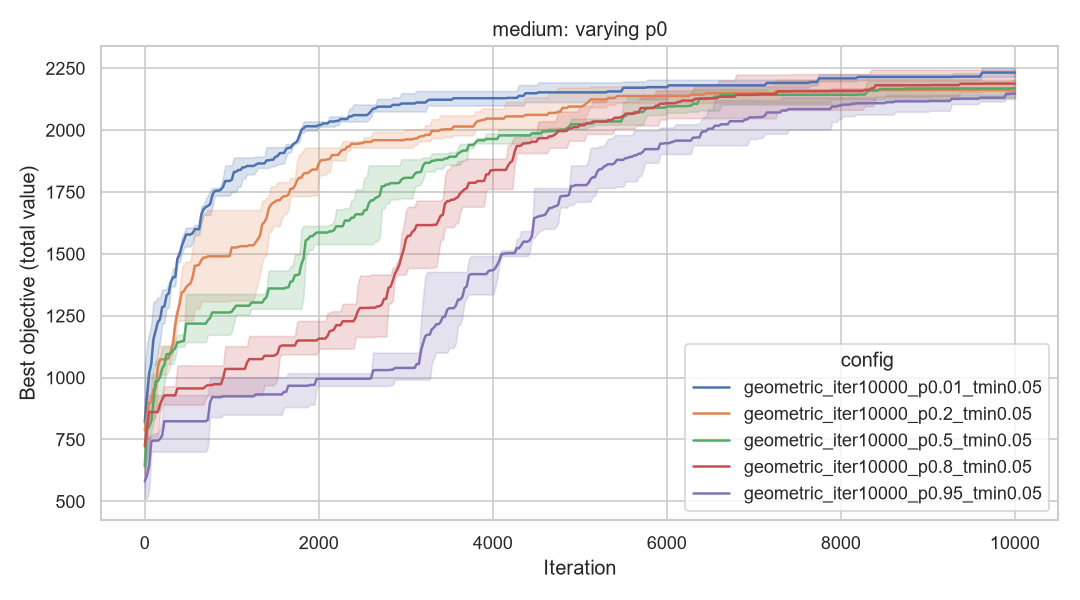
\includegraphics[width=\textwidth]{sa/medium/compare_p0.png}
		\caption{$p_0$}
	\end{subfigure}
	\begin{subfigure}{0.49\textwidth}
		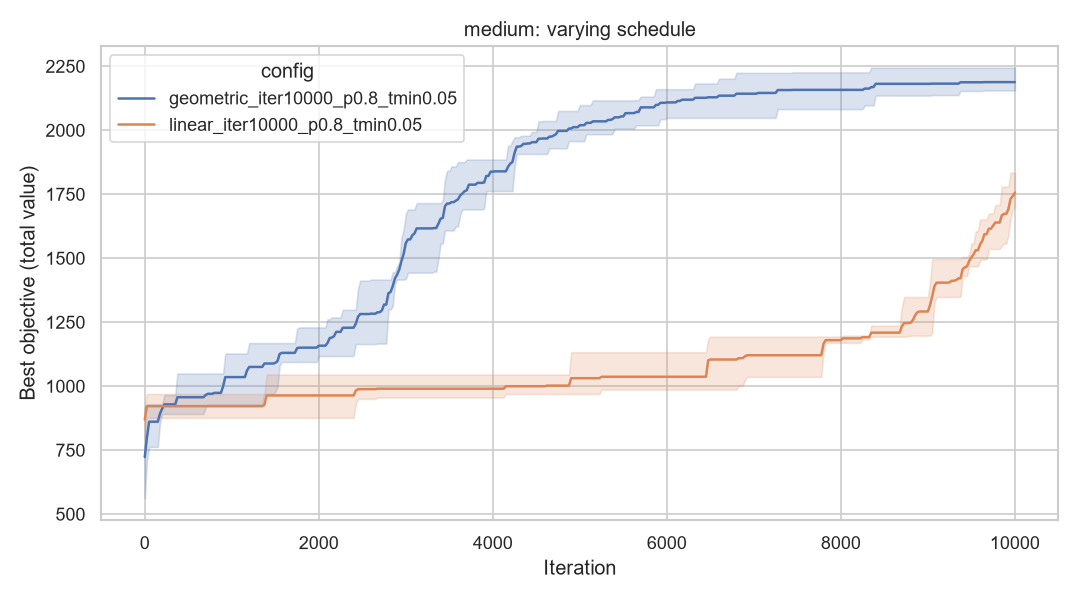
\includegraphics[width=\textwidth]{sa/medium/compare_schedule.png}
		\caption{Jadwal suhu}
	\end{subfigure}
	\begin{subfigure}{0.49\textwidth}
		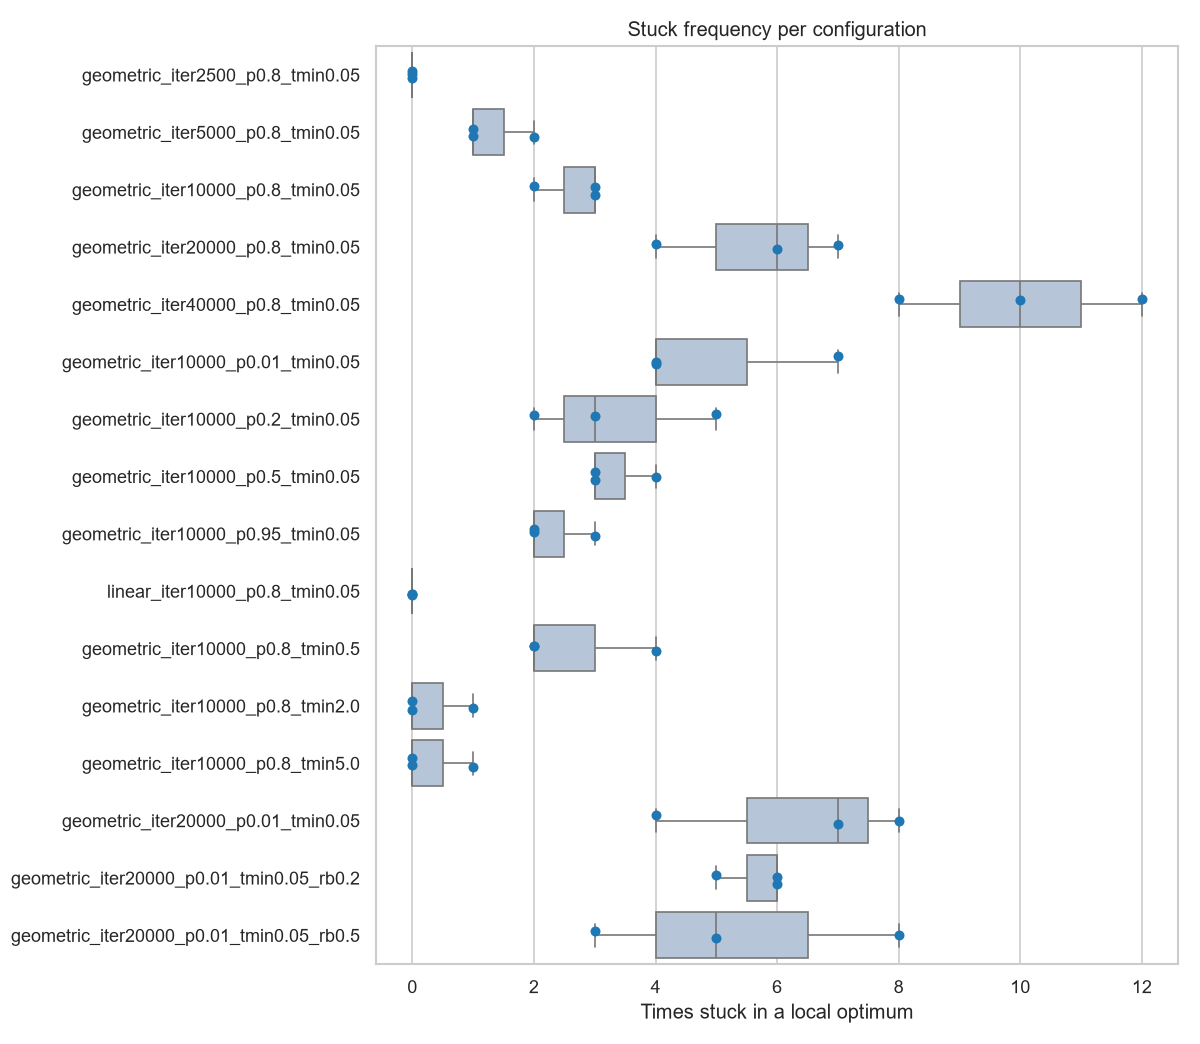
\includegraphics[width=\textwidth]{sa/medium/stuck_count_box.png}
		\caption{Frekuensi \textit{stuck}}
	\end{subfigure}
	\caption{Perbandingan konfigurasi Simulated Annealing (instans \textit{medium})}
	\label{fig:sa-compare}
\end{figure}

\begin{table}[H]\centering\small
\caption{Pengaruh \textit{ratio bias} pada instans \textit{large} (rata-rata 3 \textit{run})}\label{tab:sa-large-bias}
\begin{tabular}{r r r r r}
\toprule
\textbf{Ratio bias} & \textbf{Akhir} & \textbf{Gap (\%)} & \textbf{Durasi (s)} & \textbf{Stuck} \\
\midrule
0 & 4976.0 $\pm$ 66.9 & 11.7 & 21.5 & 8.3 \\
0.2 & 5076.3 $\pm$ 42.3 & 9.9 & 21.3 & 9.0 \\
0.5 & 5058.0 $\pm$ 74.8 & 10.2 & 19.7 & 8.0 \\
\bottomrule
\end{tabular}
\end{table}


\section{Hasil Genetic Algorithm}

Sesuai spesifikasi, dilakukan dua eksperimen: (1) populasi tetap 50 dengan
generasi 50, 100, dan 200; (2) generasi tetap 100 dengan populasi 20, 50, dan 100.
Laju mutasi 0,2 dan \textit{elitism} 1. Konfigurasi (50, 100) termasuk dalam kedua
eksperimen. Ringkasannya ada pada Tabel~\ref{tab:ga-summary}, sedangkan hasil setiap
\textit{run} (populasi, iterasi, nilai awal dan akhir, durasi) ada pada
Tabel~\ref{tab:ga-runs} di Lampiran. Kolom ``Awal'' adalah nilai individu terbaik
generasi ke-0.

\begin{table}[H]\centering\small
\caption{Ringkasan Genetic Algorithm (rata-rata 3 \textit{run})}\label{tab:ga-summary}
\begin{adjustbox}{max width=\textwidth}\begin{tabular}{l r r r r r r r r}
\toprule
\textbf{Instans} & \textbf{Pop.} & \textbf{Gen.} & \textbf{Awal} & \textbf{Akhir (mean $\pm$ std)} & \textbf{Min--maks} & \textbf{Gap (\%)} & \textbf{Durasi (s)} & \textbf{Gen. terbaik} \\
\midrule
\multirow{5}{*}{\textit{small}} & 50.0 & 50.0 & 488.3 & 608.0 $\pm$ 41.2 & 563--644 & 17.2 & 0.21 & 29.0 \\
 & 50.0 & 100.0 & 486.0 & 640.7 $\pm$ 12.0 & 629--653 & 12.7 & 0.38 & 61.0 \\
 & 50.0 & 200.0 & 380.7 & 698.3 $\pm$ 16.7 & 679--708 & 4.9 & 1.03 & 110.0 \\
 & 20.0 & 100.0 & 389.0 & 569.3 $\pm$ 26.5 & 548--599 & 22.4 & 0.20 & 64.0 \\
 & 100.0 & 100.0 & 437.0 & 655.3 $\pm$ 11.5 & 644--667 & 10.7 & 1.18 & 54.7 \\
\midrule
\multirow{5}{*}{\textit{medium}} & 50.0 & 50.0 & 1082.3 & 1221.7 $\pm$ 58.3 & 1186--1289 & 48.8 & 0.15 & 24.3 \\
 & 50.0 & 100.0 & 992.0 & 1319.3 $\pm$ 211.7 & 1154--1558 & 44.7 & 0.34 & 90.3 \\
 & 50.0 & 200.0 & 1034.7 & 1477.7 $\pm$ 105.2 & 1369--1579 & 38.0 & 0.67 & 185.3 \\
 & 20.0 & 100.0 & 975.0 & 1220.0 $\pm$ 98.1 & 1120--1316 & 48.8 & 0.13 & 89.7 \\
 & 100.0 & 100.0 & 993.3 & 1422.7 $\pm$ 78.7 & 1353--1508 & 40.3 & 0.63 & 91.3 \\
\midrule
\multirow{5}{*}{\textit{large}} & 50.0 & 50.0 & 2030.0 & 2080.0 $\pm$ 17.7 & 2064--2099 & 63.1 & 0.98 & 27.3 \\
 & 50.0 & 100.0 & 2074.7 & 2115.0 $\pm$ 245.5 & 1932--2394 & 62.5 & 2.42 & 14.0 \\
 & 50.0 & 200.0 & 1983.7 & 2096.3 $\pm$ 220.9 & 1923--2345 & 62.8 & 6.37 & 187.0 \\
 & 20.0 & 100.0 & 2070.0 & 2211.0 $\pm$ 112.9 & 2130--2340 & 60.7 & 1.29 & 91.3 \\
 & 100.0 & 100.0 & 2181.0 & 2265.7 $\pm$ 193.5 & 2071--2458 & 59.8 & 10.69 & 57.0 \\
\bottomrule
\end{tabular}\end{adjustbox}
\end{table}


\begin{figure}[H]
	\centering
	\begin{subfigure}{0.49\textwidth}
		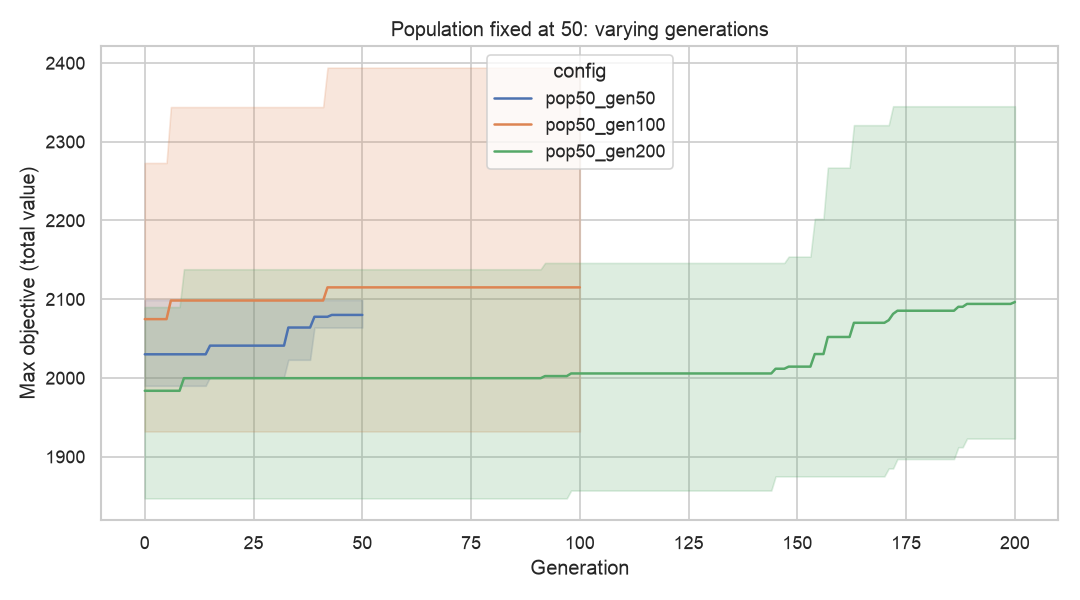
\includegraphics[width=\textwidth]{ga/large/compare_generations.png}
		\caption{Populasi 50, generasi bervariasi}
	\end{subfigure}
	\begin{subfigure}{0.49\textwidth}
		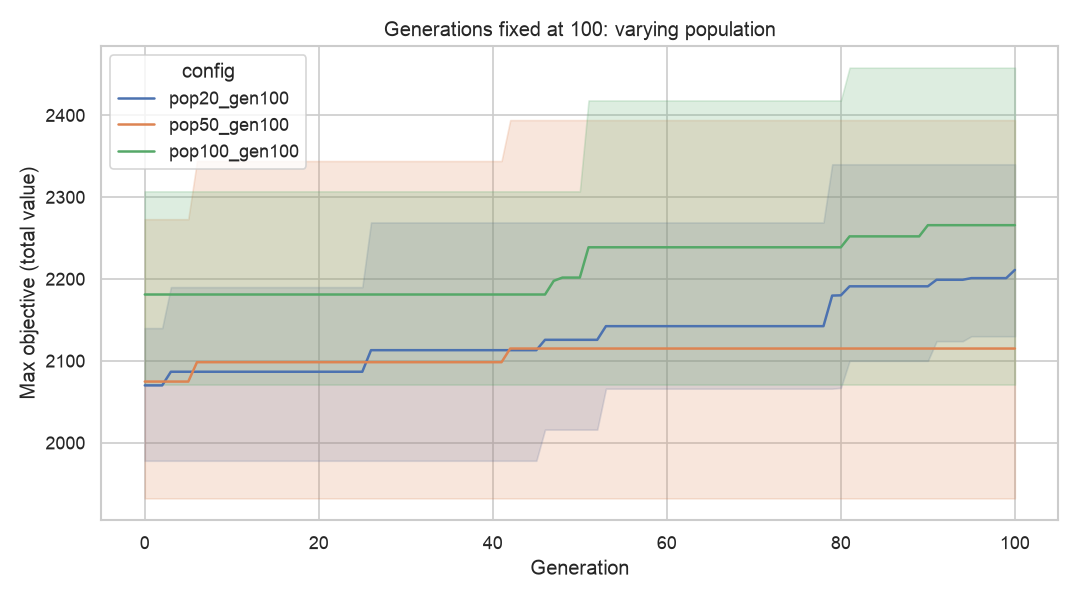
\includegraphics[width=\textwidth]{ga/large/compare_population.png}
		\caption{Generasi 100, populasi bervariasi}
	\end{subfigure}
	\caption{Nilai objektif maksimum GA terhadap generasi (instans \textit{large}; garis = rata-rata 3 \textit{run}, area = rentang)}
	\label{fig:ga-compare}
\end{figure}

\begin{figure}[H]
	\centering
	\begin{subfigure}{0.49\textwidth}
		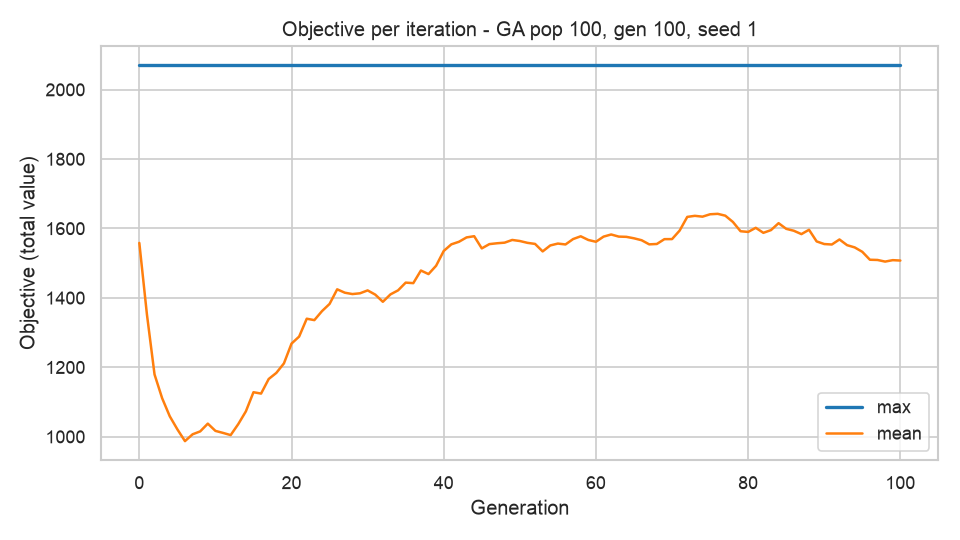
\includegraphics[width=\textwidth]{ga/large/pop100_gen100/seed1/curve.png}
		\caption{Nilai maksimum dan rata-rata populasi}
	\end{subfigure}
	\begin{subfigure}{0.49\textwidth}
		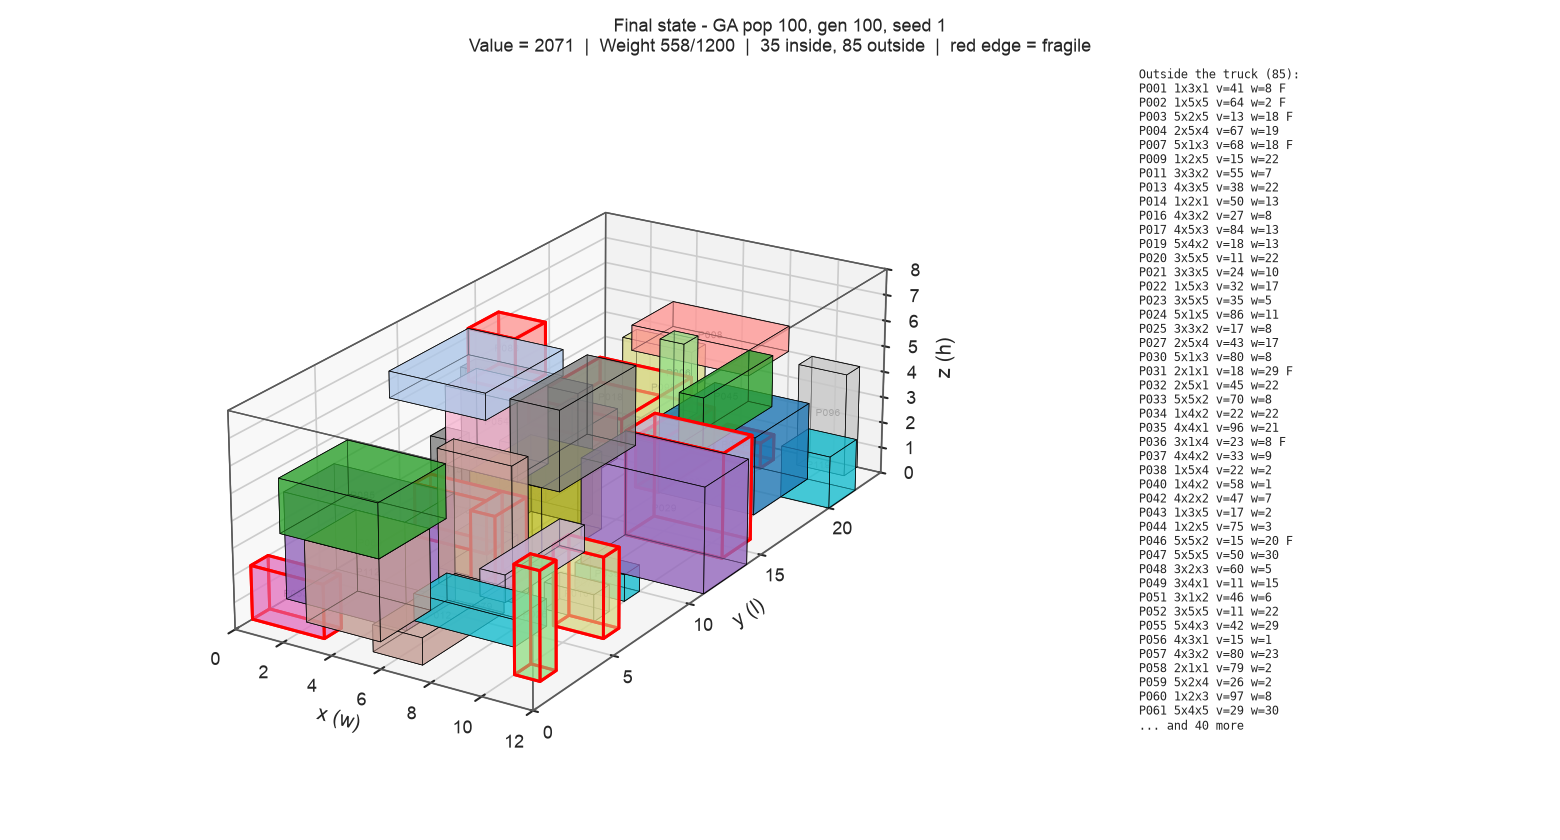
\includegraphics[width=\textwidth]{ga/large/pop100_gen100/seed1/final.png}
		\caption{\textit{State} akhir}
	\end{subfigure}
	\caption{GA populasi 100, generasi 100 (instans \textit{large}, \textit{seed} 1)}
	\label{fig:ga-run}
\end{figure}

\section{Hasil Bonus: Objektif ETA}

SA (jadwal geometrik, 20.000 iterasi, $p_0=0{,}01$, \textit{seed} 1) dijalankan pada
instans \textit{medium} dengan objektif ETA dan objektif \textit{value} biasa
(\texttt{output/sa/medium/eta/}).

\begin{table}[H]
	\centering
	\caption{Perbandingan objektif \textit{value} dan ETA (SA, instans \textit{medium}, \textit{seed} 1)}
	\label{tab:eta}
	\begin{tabular}{l r r r r}
		\toprule
		\textbf{Objektif} & \textbf{Total value} & $\sum$ \textbf{value/ETA} & \textbf{Paket dimuat} & \textbf{Rata-rata ETA} \\
		\midrule
		\textit{value} & 2266 & 933,4 & 40 & 3,95 \\
		ETA & 2180 & 966,0 & 40 & 3,70 \\
		\bottomrule
	\end{tabular}
\end{table}

Objektif ETA mengorbankan 3,8\% total \textit{value} untuk memuat paket dengan rata-rata
ETA lebih kecil (3,70 dibanding 3,95 hari; rata-rata ETA semua paket 4,11). Artinya,
paket yang lebih mendesak lebih diprioritaskan, sesuai tujuan objektif ini.

\section{Hasil Bonus: Multi-Truk}
\label{sec:multitruck-hasil}

Armada dua truk identik diuji pada instans \textit{medium} dan \textit{large} dengan
parameter yang sama seperti eksperimen satu truk (3 \textit{run} per konfigurasi;
hasilnya ada di \texttt{output/*/medium\_trucks2/} dan \texttt{output/*/large\_trucks2/}).
HC hanya dijalankan untuk \textit{steepest} dan \textit{stochastic} di \textit{medium}
karena waktu eksekusinya. Untuk kedua instans, total berat dan volume seluruh paket
muat di dua truk, sehingga batas atasnya sama dengan total \textit{value} semua paket
(2608 dan 6194). Seluruh 42 \textit{state} akhir diperiksa ulang dengan pemeriksa
independen berbasis sel, dan semuanya valid.

\begin{table}[H]
	\centering
	\caption{Hasil multi-truk dibanding satu truk (rata-rata 3 \textit{run})}
	\label{tab:multitruck}
	\begin{adjustbox}{max width=\textwidth}
	\begin{tabular}{l l r r r r}
		\toprule
		\textbf{Instans} & \textbf{Algoritma} & \textbf{1 truk} & \textbf{2 truk (mean $\pm$ std)} & \textbf{Gap 2 truk (\%)} & \textbf{Durasi 2 truk (s)} \\
		\midrule
		\multirow{5}{*}{\textit{medium}} & HC \textit{steepest} & 2213,7 & 2544,3 $\pm$ 6,5 & 2,4 & 48,1 \\
		& HC \textit{stochastic} & 2105,3 & 2426,0 $\pm$ 51,6 & 7,0 & 23,7 \\
		& SA (20.000 iterasi, $p_0=0{,}01$) & 2233,3 & 2543,0 $\pm$ 28,0 & 2,5 & 4,6 \\
		& GA (pop. 50, gen. 100) & 1319,3 & 1608,7 $\pm$ 66,3 & 38,3 & 0,7 \\
		& GA (pop. 50, gen. 200) & 1477,7 & 1691,7 $\pm$ 68,0 & 35,1 & 1,3 \\
		\midrule
		\multirow{3}{*}{\textit{large}} & SA (20.000 iterasi, $p_0=0{,}01$) & 4976,0 & 5921,7 $\pm$ 27,2 & 4,4 & 12,2 \\
		& GA (pop. 50, gen. 100) & 2115,0 & 2598,7 $\pm$ 47,5 & 58,0 & 1,0 \\
		& GA (pop. 50, gen. 200) & 2096,3 & 2873,0 $\pm$ 244,4 & 53,6 & 2,2 \\
		\bottomrule
	\end{tabular}
	\end{adjustbox}
\end{table}

\begin{figure}[H]
	\centering
	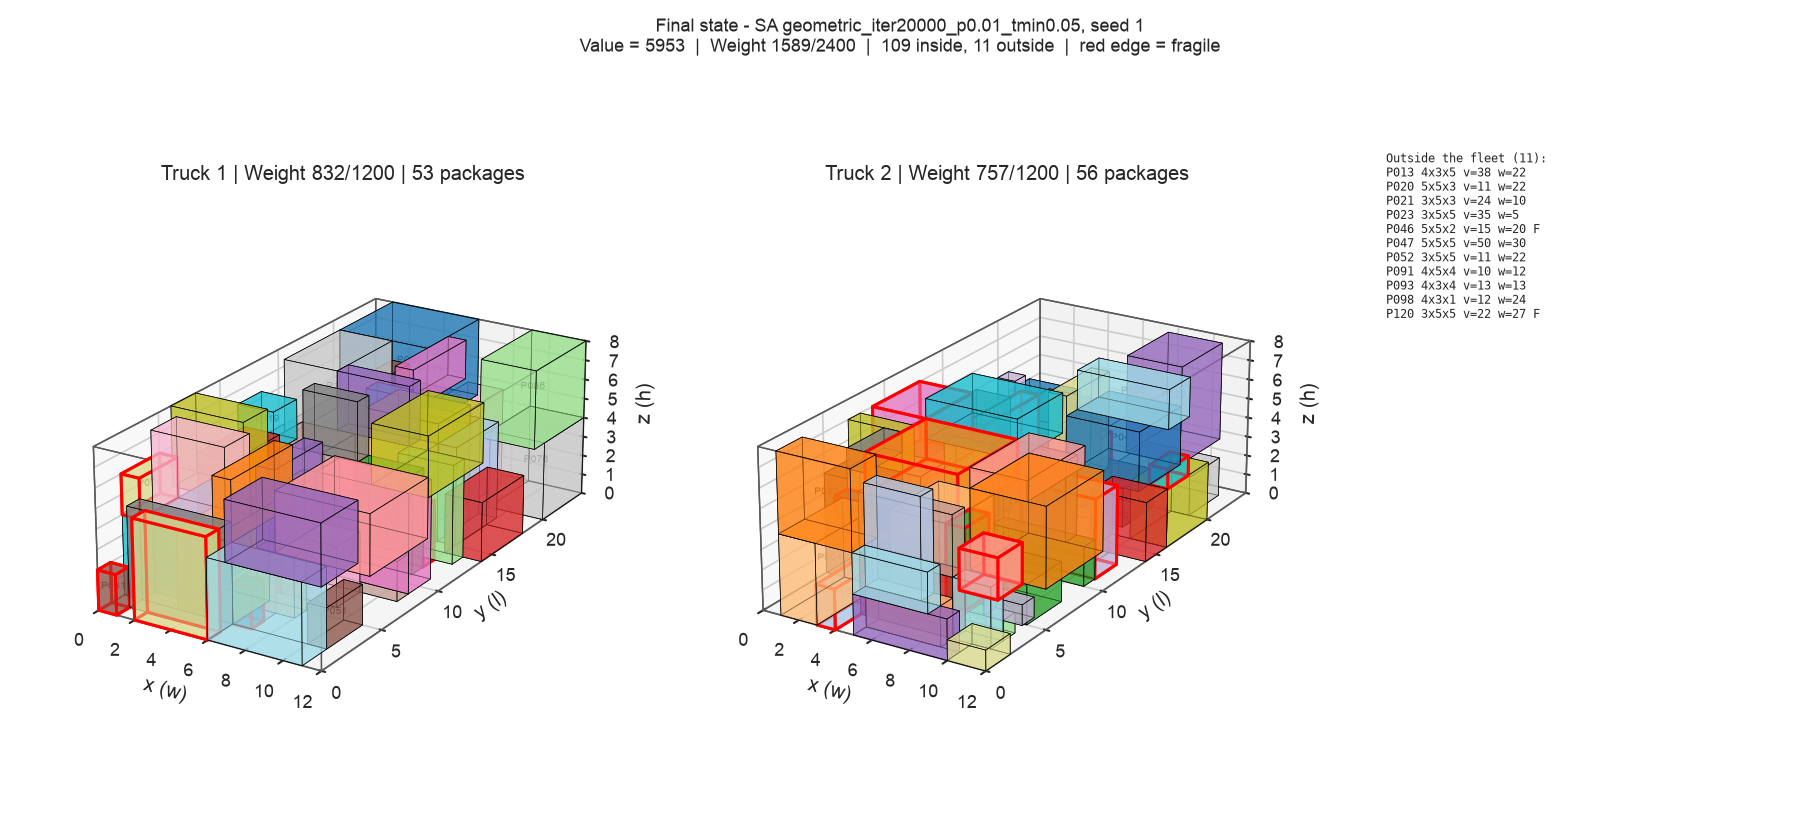
\includegraphics[width=\textwidth]{sa/large_trucks2/geometric_iter20000_p0.01_tmin0.05/seed1/final.png}
	\caption{\textit{State} akhir SA dengan dua truk (instans \textit{large}, \textit{seed} 1)}
	\label{fig:multitruck}
\end{figure}

Dengan dua truk, total \textit{value} yang diangkut naik 14--19\% untuk HC dan SA.
Kenaikannya tidak 100\% karena sebagian besar paket bernilai tinggi sudah terangkut
oleh satu truk. Pada \textit{large}, batasnya bukan lagi berat (1589 dari 2400 pada
Gambar~\ref{fig:multitruck}), melainkan volume dan geometri: paket yang tersisa di luar
umumnya berukuran besar dengan \textit{value} kecil. HC \textit{steepest} dan SA kini
hanya 2--4\% dari batas atas. Urutan kinerja algoritma tetap sama seperti pada satu
truk: SA dan HC \textit{steepest} unggul, HC \textit{stochastic} sedikit di bawahnya
(gap 7\%), sedangkan GA tertinggal jauh karena alasan yang sama
(Subbab~\ref{sec:ga-analisis}). Durasi SA
dan GA hanya naik sedikit, karena biaya per iterasi bergantung pada banyak paket di
setiap truk, bukan pada banyak truk.

\section{Analisis}

\begin{table}[H]
	\centering
	\caption{Perbandingan konfigurasi terbaik tiap algoritma (rata-rata 3 \textit{run})}
	\label{tab:compare}
	\begin{tabular}{l l r r r}
		\toprule
		\textbf{Instans} & \textbf{Algoritma} & \textbf{Akhir} & \textbf{Gap (\%)} & \textbf{Durasi (s)} \\
		\midrule
		\multirow{4}{*}{\textit{small}}  & HC \textit{steepest} & 680,7 & 7,3 & 0,29 \\
		& HC \textit{random-restart} & 712,7 & 2,9 & 1,21 \\
		& SA (20.000 iterasi) & \textbf{734,0} & \textbf{0,0} & 4,63 \\
		& GA (pop. 50, gen. 200) & 698,3 & 4,9 & 1,00 \\
		\midrule
		\multirow{5}{*}{\textit{medium}} & HC \textit{steepest} & 2213,7 & 7,1 & 53,51 \\
		& HC \textit{random-restart} & 2260,7 & 5,2 & 120,72 \\
		& SA (20.000 iterasi, $p_0=0{,}01$) & 2233,3 & 6,3 & 23,04 \\
		& SA (40.000 iterasi, $p_0=0{,}8$) & \textbf{2262,3} & \textbf{5,1} & 37,29 \\
		& GA (pop. 50, gen. 200) & 1477,7 & 38,0 & 0,67 \\
		\midrule
		\multirow{4}{*}{\textit{large}}  & HC \textit{steepest} & 5205,7 & 7,6 & 693,51 \\
		& HC \textit{random-restart} & \textbf{5261,7} & \textbf{6,6} & 1683,70 \\
		& SA (20.000 iterasi, \textit{ratio bias} 0,2) & 5076,3 & 9,9 & 21,30 \\
		& GA (pop. 100, gen. 100) & 2265,7 & 59,8 & 10,70 \\
		\bottomrule
	\end{tabular}
\end{table}

\subsection{Seberapa dekat dengan optimum global?}

Pada instans \textit{small}, SA mencapai 734 pada ketiga \textit{run}. Nilai ini sama
dengan batas atas, sehingga hasil SA \emph{terbukti} merupakan optimum global.
HC \textit{random-restart} tertinggal 2,9\% dan GA 4,9\%. Pada \textit{medium} dan
\textit{large}, HC dan SA berada 5--10\% di bawah batas atas (HC \textit{stochastic}
12--18\%). Angka ini merupakan
batas atas jarak, karena batas atas \textit{knapsack} mengabaikan geometri:
kombinasi paket yang muat berdasarkan berat dan volume belum tentu dapat disusun
tanpa celah, tanpa melayang, dan tanpa bertumpu pada paket \textit{fragile}.
Jarak sebenarnya ke optimum global kemungkinan lebih kecil.

GA tertinggal jauh pada \textit{medium} (38\%) dan \textit{large} (60\%). Penyebabnya
dibahas pada Subbab~\ref{sec:ga-analisis}.

\subsection{Perbandingan antaralgoritma}

\begin{itemize}
	\item \textbf{HC \textit{steepest-ascent}} cepat naik pada awal pencarian
	(Gambar~\ref{fig:hc-curve}), tetapi berhenti di \textit{local optimum} setelah
	7--65 iterasi. Hasilnya sudah cukup baik karena setiap langkah memilih yang terbaik
	dari ribuan tetangga.
	\item \textbf{HC \textit{stochastic}} hasilnya 0,5--11\% di bawah \textit{steepest}
	(gap 8--18\%) dengan waktu lebih singkat (0,1 detik di \textit{small}, 19 detik di
	\textit{medium}, dan 10 menit di \textit{large}). Langkahnya acak di antara tetangga
	yang lebih baik, bukan yang terbaik, sehingga setiap langkah naik lebih sedikit dan
	puncak yang dicapai umumnya lebih rendah. Pada \textit{large}, dua dari tiga
	\textit{run} berhenti karena \texttt{max\_iterations}=100, sehingga hasilnya masih
	dapat naik dengan iterasi lebih banyak.
	\item \textbf{HC \textit{sideways move}} tidak lebih baik daripada \textit{steepest}.
	Semua \textit{run} berhenti karena batas \textit{sideways move}. Artinya banyak
	\textit{plateau} (misalnya rotasi atau \textit{swap} paket di luar truk yang tidak
	mengubah nilai), tetapi berjalan di \textit{plateau} jarang menemukan jalan naik.
	\item \textbf{HC \textit{random-restart}} adalah varian HC terbaik dan paling konsisten,
	dengan biaya waktu beberapa kali lipat \textit{steepest} karena setiap
	\textit{restart} adalah satu pendakian penuh.
	\item \textbf{SA} terbaik di \textit{small}, setara HC \textit{random-restart} di
	\textit{medium} bila diberi 40.000 iterasi, dan sedikit di bawahnya di \textit{large}.
	Keunggulannya adalah waktu: puluhan detik dibanding puluhan menit HC pada \textit{large}.
	\item \textbf{GA} terburuk pada instans sedang dan besar meskipun waktunya singkat.
\end{itemize}

\subsection{Perbandingan durasi}

Biaya HC \textit{steepest} dan \textit{sideways} per iterasi sebanding dengan banyak
tetangga, yaitu $O(n^2)$ \textit{swap} ditambah $O(n^2)$ \textit{move} ke \textit{extreme
point}. Setiap tetangga juga di-\textit{repair}, yang biayanya kuadratik terhadap banyak
paket di truk. Karena itu waktunya tumbuh sangat cepat: sekitar 0,3 detik di
\textit{small}, 50 detik di \textit{medium}, dan 10--16 menit di \textit{large}.
\textit{Random-restart} sekitar 2--2,5 kali \textit{steepest}. HC \textit{stochastic}
hanya memeriksa seluruh tetangga ketika 50 tetangga acak tidak memberi perbaikan.
Pada satu \textit{run} \textit{medium}, hal ini terjadi pada 16 dari 36 iterasi dan
menghabiskan 98\% waktunya. Karena itu durasinya lebih singkat daripada
\textit{steepest}, tetapi tumbuh dengan cara yang sama terhadap ukuran instans.
Sebaliknya, SA dan GA hanya
menilai satu tetangga per iterasi atau per anak, sehingga biayanya hampir linear
terhadap banyak iterasi (Tabel~\ref{tab:sa-params}: 2.500 iterasi 1,7 detik, 40.000
iterasi 37 detik). GA paling cepat karena total anak yang dievaluasi hanya
populasi $\times$ generasi (paling banyak 10.000).

% TODO: hapus catatan ini jika eksperimen SA dijalankan ulang pada mesin yang sama dengan HC dan GA.
Catatan: eksperimen SA dijalankan pada waktu yang berbeda dari eksperimen HC dan GA.
Pengukuran ulang satu \textit{run} SA \textit{medium} 20.000 iterasi pada mesin yang
sama dengan HC hanya memerlukan sekitar 3 detik (Tabel~\ref{tab:sa-runs} mencatat
sekitar 23 detik). Karena itu, perbandingan durasi antaralgoritma dibaca sebagai
orde besaran. Kesimpulan bahwa HC jauh lebih lambat daripada SA pada instans besar
tidak berubah.

\subsection{Konsistensi hasil}

SA pada \textit{small} memberikan hasil identik di ketiga \textit{run}. Pada
\textit{medium} dan \textit{large}, HC \textit{random-restart} paling konsisten
(simpangan baku 7 dan 46), disusul SA (21 dan 42--75) dan HC \textit{steepest}.
HC \textit{stochastic} kurang konsisten (simpangan baku 54--123) karena langkahnya
dipilih secara acak, dan GA paling tidak konsisten. Simpangan baku GA mencapai
245 pada \textit{large}, karena hasilnya sangat bergantung pada individu awal terbaik
yang kebetulan terbentuk.

\subsection{Pengaruh parameter Simulated Annealing}

\begin{itemize}
	\item \textbf{Banyak iterasi} adalah parameter paling berpengaruh: nilai akhir naik
	dari 1985,7 (2.500 iterasi) menjadi 2262,3 (40.000 iterasi). Frekuensi \textit{stuck}
	ikut naik, karena dengan jadwal yang lebih panjang lebih banyak waktu dihabiskan
	pada suhu rendah.
	\item \textbf{$p_0$ kecil (0,01)} memberi hasil terbaik pada 10.000 iterasi. Dengan
	$p_0$ besar, sebagian besar iterasi awal terbuang untuk menerima langkah buruk.
	Karena setiap \textit{state} sudah di-\textit{repair} menjadi valid, sehingga eksplorasi
	berlebihan tidak diperlukan.
	\item \textbf{Jadwal geometrik} jauh lebih baik daripada linear (2187,7 vs 1755,7).
	Jadwal linear mempertahankan suhu tinggi terlalu lama dan baru dingin di akhir,
	sehingga waktu untuk memperbaiki solusi sangat sedikit.
	\item \textbf{$T_{\min}$ kecil} lebih baik. Dengan $T_{\min}=5$, langkah memburuk masih
	sering diterima di akhir, sehingga solusi tidak sempat ``mengeras''.
	\item \textbf{\textit{Ratio bias}} sedikit menaikkan rata-rata, yaitu +0,6\% di
	\textit{medium} dan +2,0\% di \textit{large} untuk bias 0,2.
\end{itemize}

\subsection{Pengaruh populasi dan generasi pada Genetic Algorithm}
\label{sec:ga-analisis}

Pada \textit{small} dan \textit{medium}, menambah generasi (50 $\rightarrow$ 200) dan
menambah populasi (20 $\rightarrow$ 100) sama-sama menaikkan nilai akhir. Pada
\textit{medium} nilainya naik dari 1221,7 ke 1477,7 untuk generasi dan dari 1220,0 ke
1422,7 untuk populasi. Kurva pada Gambar~\ref{fig:ga-compare} masih naik di akhir,
sehingga GA belum konvergen. Durasi naik linear terhadap populasi $\times$ generasi.
Pada \textit{large}, pengaruh keduanya hampir tertutup oleh variansi: banyak
\textit{run} tidak pernah melampaui individu terbaik generasi ke-0 (kolom ``Gen.
terbaik'' bernilai 0 pada Tabel~\ref{tab:ga-runs}).

Rendahnya kinerja GA disebabkan oleh operator \textit{crossover}. \textit{Single-point
crossover} menggabungkan koordinat paket dari dua susunan yang tidak berhubungan.
Posisi yang baik pada satu induk hanya bermakna relatif terhadap paket lain di susunan
induk itu, sehingga anak umumnya berisi banyak paket yang bertumpuk. \textit{Repair}
kemudian mengeluarkan paket-paket tersebut. Pengukuran tambahan pada 200 pasangan induk
acak dari populasi awal menunjukkan bahwa anak (setelah \textit{repair}) lebih baik
daripada induk terbaiknya hanya pada 8\% (\textit{small}), 6\% (\textit{medium}), dan
2\% (\textit{large}) kasus. Perbaikan nilai praktis hanya berasal dari mutasi, yaitu
satu langkah per anak dengan peluang 0,2. Jumlah ini jauh lebih sedikit daripada
puluhan ribu langkah SA. Selain itu, populasi awal acak setelah \textit{repair} hanya
berisi sekitar separuh paket yang semula dimasukkan, sehingga titik awal GA rendah.
Representasi yang cocok untuk \textit{crossover} versi salindia (\textit{string} dengan
gen yang independen, seperti 8-\textit{queens}) tidak cocok untuk persoalan
\textit{packing} yang gennya saling bergantung secara geometris.


	\chapter{Kesimpulan dan Saran}
	\section{Kesimpulan}

\begin{enumerate}
	\item Ketiga algoritma \textit{local search} (Hill-Climbing dengan keempat variannya,
	Simulated Annealing, dan Genetic Algorithm) berhasil diimplementasikan untuk
	persoalan pengisian peti kemas truk. Seluruh solusi akhir memenuhi batasan dinding,
	tumpang tindih, tumpuan, \textit{fragile}, dan kapasitas berkat heuristik
	\textit{repair}.
	\item Simulated Annealing memberikan keseimbangan terbaik antara kualitas dan waktu.
	SA mencapai optimum global (terbukti oleh batas atas \textit{knapsack}) pada instans
	\textit{small} di ketiga \textit{run}, dan berada 5--10\% dari batas atas pada
	instans yang lebih besar dalam hitungan detik.
	\item HC \textit{random-restart} memberikan hasil terbaik dan paling konsisten pada
	instans \textit{medium} dan \textit{large}, tetapi waktunya paling lama (sekitar 28
	menit per \textit{run} pada \textit{large}) karena membangkitkan seluruh tetangga di
	setiap iterasi. HC \textit{stochastic} paling cepat tetapi paling mudah terjebak.
	\item Genetic Algorithm versi salindia (\textit{roulette wheel}, \textit{single-point
	crossover}, mutasi) bekerja cukup baik pada instans kecil, tetapi tertinggal jauh pada
	instans sedang dan besar. \textit{Crossover} yang menukar ekor kromosom merusak susunan
	geometris yang dibangun induk. Menambah populasi dan generasi tetap meningkatkan
	hasil, tetapi tidak menutup selisih tersebut.
	\item Parameter terpenting SA adalah banyak iterasi dan jadwal suhu. Jadwal geometrik
	dengan $p_0$ dan $T_{\min}$ kecil memberikan hasil terbaik.
	\item Objektif alternatif berbasis ETA berhasil menggeser pilihan paket ke paket yang
	lebih mendesak dengan pengorbanan total \textit{value} yang kecil (3,8\%).
	\item Dukungan multi-truk diperoleh hanya dengan menambahkan identitas truk pada
	\textit{state} serta memeriksa batasan per truk, tanpa mengubah ketiga algoritma.
	Dengan dua truk, SA dan HC \textit{steepest} mengangkut 14--19\% lebih banyak
	\textit{value} dan berada 2--4\% dari batas atas.
\end{enumerate}

\section{Saran}

\begin{enumerate}
	\item \textbf{Representasi GA berbasis urutan.} Kromosom dapat diubah menjadi urutan
	paket beserta orientasinya, lalu didekode secara \textit{greedy} ke \textit{extreme
	point} pertama yang valid. Dengan \textit{order crossover}, anak selalu berupa susunan
	valid yang mewarisi urutan prioritas induknya.
	\item \textbf{Inisialisasi dan pengisian \textit{greedy}.} Uji coba awal di luar kode
	utama, yaitu menambahkan langkah pengisian \textit{greedy} ke \textit{extreme point}
	setelah \textit{repair}, menaikkan rata-rata GA (populasi 50, generasi 100) dari
	sekitar 1439 menjadi 2313 pada \textit{medium} dan dari 2302 menjadi 5370 pada
	\textit{large}. Sebagian besar kenaikan berasal dari heuristik \textit{greedy} itu
	sendiri, sehingga pendekatan ini perlu dikaji sebagai algoritma memetik.
	\item \textbf{Evaluasi inkremental.} \textit{Repair} dan pemeriksaan batasan saat ini
	menghitung ulang seluruh \textit{state} untuk setiap tetangga. Evaluasi inkremental
	(hanya memeriksa paket yang berubah) akan mempercepat HC \textit{steepest} secara
	signifikan.
	\item \textbf{Eksekusi paralel.} \textit{Run} antar-\textit{seed} dan antarkonfigurasi
	independen, sehingga eksperimen dapat dijalankan paralel. Pengukuran durasi
	sebaiknya tetap dilakukan dalam kondisi yang sama untuk semua algoritma.
\end{enumerate}


	\chapter{Pembagian Tugas}
	\begin{table}[H]
	\centering
	\caption{Pembagian tugas anggota kelompok}
	\label{tab:pembagian}
	\begin{tabular}{l l l}
		\toprule
		\textbf{Nama} & \textbf{NIM} & \textbf{Tugas} \\
		\midrule
		Athilla Zaidan Zidna Fann & 13524068 & Genetic Algorithm \\
		Jason Edward Salim & 13524034 & Simulated Annealing \\
		Raynard Fausta & 13524052 & Hill-Climbing, multi-truk (bonus) \\
		\bottomrule
	\end{tabular}
\end{table}


	\bibliography{dafpus}

	\appendix
	\chapter{Lampiran}
	\section{Tautan Repository}

\url{https://github.com/AthillaZaidan/IF3170_G04_BUMC}

\section{Hasil Setiap Run Genetic Algorithm}

{\scriptsize\setlength{\tabcolsep}{4pt}
\begin{longtable}{r r c r r r r}
\caption{Hasil setiap \textit{run} Genetic Algorithm}\label{tab:ga-runs}\\
\toprule
\textbf{Pop.} & \textbf{Gen.} & \textbf{Seed} & \textbf{Awal} & \textbf{Akhir} & \textbf{Durasi (s)} & \textbf{Gen. terbaik} \\
\endfirsthead
\toprule
\textbf{Pop.} & \textbf{Gen.} & \textbf{Seed} & \textbf{Awal} & \textbf{Akhir} & \textbf{Durasi (s)} & \textbf{Gen. terbaik} \\
\endhead
\midrule
\multicolumn{7}{l}{\textit{small}} \\
50 & 50 & 1 & 470 & 563 & 0.10 & 15 \\
50 & 50 & 2 & 477 & 617 & 0.19 & 27 \\
50 & 50 & 3 & 518 & 644 & 0.34 & 45 \\
50 & 100 & 1 & 486 & 653 & 0.34 & 39 \\
50 & 100 & 2 & 506 & 629 & 0.44 & 77 \\
50 & 100 & 3 & 466 & 640 & 0.37 & 67 \\
50 & 200 & 1 & 343 & 708 & 0.87 & 120 \\
50 & 200 & 2 & 379 & 679 & 1.13 & 111 \\
50 & 200 & 3 & 420 & 708 & 1.09 & 99 \\
20 & 100 & 1 & 396 & 548 & 0.23 & 35 \\
20 & 100 & 2 & 382 & 599 & 0.21 & 70 \\
20 & 100 & 3 & 389 & 561 & 0.16 & 87 \\
100 & 100 & 1 & 446 & 655 & 1.20 & 55 \\
100 & 100 & 2 & 410 & 667 & 1.00 & 68 \\
100 & 100 & 3 & 455 & 644 & 1.35 & 41 \\
\midrule
\multicolumn{7}{l}{\textit{medium}} \\
50 & 50 & 1 & 980 & 1190 & 0.15 & 44 \\
50 & 50 & 2 & 1289 & 1289 & 0.16 & 0 \\
50 & 50 & 3 & 978 & 1186 & 0.14 & 29 \\
50 & 100 & 1 & 970 & 1246 & 0.34 & 91 \\
50 & 100 & 2 & 1015 & 1558 & 0.36 & 88 \\
50 & 100 & 3 & 991 & 1154 & 0.31 & 92 \\
50 & 200 & 1 & 983 & 1485 & 0.64 & 192 \\
50 & 200 & 2 & 1115 & 1369 & 0.69 & 166 \\
50 & 200 & 3 & 1006 & 1579 & 0.67 & 198 \\
20 & 100 & 1 & 947 & 1120 & 0.14 & 97 \\
20 & 100 & 2 & 1047 & 1316 & 0.12 & 82 \\
20 & 100 & 3 & 931 & 1224 & 0.15 & 90 \\
100 & 100 & 1 & 964 & 1508 & 0.67 & 94 \\
100 & 100 & 2 & 1029 & 1407 & 0.61 & 99 \\
100 & 100 & 3 & 987 & 1353 & 0.60 & 81 \\
\midrule
\multicolumn{7}{l}{\textit{large}} \\
50 & 50 & 1 & 2099 & 2099 & 1.02 & 0 \\
50 & 50 & 2 & 2001 & 2077 & 0.78 & 43 \\
50 & 50 & 3 & 1990 & 2064 & 1.15 & 39 \\
50 & 100 & 1 & 1932 & 1932 & 2.27 & 0 \\
50 & 100 & 2 & 2273 & 2394 & 2.47 & 42 \\
50 & 100 & 3 & 2019 & 2019 & 2.52 & 0 \\
50 & 200 & 1 & 2014 & 2021 & 6.55 & 200 \\
50 & 200 & 2 & 2090 & 2345 & 6.77 & 172 \\
50 & 200 & 3 & 1847 & 1923 & 5.80 & 189 \\
20 & 100 & 1 & 2092 & 2163 & 1.56 & 100 \\
20 & 100 & 2 & 1978 & 2130 & 1.18 & 95 \\
20 & 100 & 3 & 2140 & 2340 & 1.13 & 79 \\
100 & 100 & 1 & 2071 & 2071 & 8.09 & 0 \\
100 & 100 & 2 & 2307 & 2458 & 12.91 & 81 \\
100 & 100 & 3 & 2165 & 2268 & 11.07 & 90 \\
\bottomrule
\end{longtable}
}


\section{Pernyataan Penggunaan AI Generatif}

Kelompok menggunakan asisten AI generatif selama pengerjaan tugas ini. Seluruh keluaran
AI telah diperiksa, dijalankan, dan dipahami oleh anggota kelompok.

\begin{table}[H]
	\centering
	\caption{Penggunaan AI generatif}
	\label{tab:genai}
	\begin{tabular}{p{2.5cm} p{10.7cm}}
		\toprule
		\textbf{Alat} & \textbf{Penggunaan} \\
		\midrule
		Claude & Mempelajari secara lebih mendalam cara kerja ketiga algoritma
		(Hill-Climbing, Simulated Annealing, dan Genetic Algorithm). \\
		\bottomrule
	\end{tabular}
\end{table}


\end{document}
